
\documentclass[submit]{harvardml}

% Put in your full name and email address.
\name{Weiyi Chen}
\email{wec427@g.harvard.edu}

% List any people you worked with.
\collaborators{%
    Ilias Konsoulas
}

% You don't need to change these.
\course{CS181-S16}
\assignment{Assignment \#4}
\duedate{5:00pm Feb 1, 2016}

\usepackage[OT1]{fontenc}
\usepackage[colorlinks,citecolor=blue,urlcolor=blue]{hyperref}
\usepackage[pdftex]{graphicx}
\usepackage{subfig}
\usepackage{fullpage}
\usepackage{palatino}
\usepackage{mathpazo}
\usepackage{amsmath}
\usepackage{amssymb}
\usepackage{color}
\usepackage{todonotes}
\usepackage{listings}
\usepackage{common}
\usepackage{bm}

\usepackage[mmddyyyy,hhmmss]{datetime}

\definecolor{verbgray}{gray}{0.9}

\lstnewenvironment{csv}{%
  \lstset{backgroundcolor=\color{verbgray},
  frame=single,
  framerule=0pt,
  basicstyle=\ttfamily,
  columns=fullflexible}}{}

\begin{document}
\begin{center}
{\Large Homework 4: Clustering}\\
\end{center}

There is a mathematical component and a programming component to this homework.
Please submit ONLY your PDF to Canvas, and push all of your work to your Github
repository. If a question requires you to make any plots, please
include those in the writeup.


%%%%%%%%%%%%%%%%%%%%%%%%%%%%%%%%%%%%%%%%%%%%%
% Problem 1
%%%%%%%%%%%%%%%%%%%%%%%%%%%%%%%%%%%%%%%%%%%%%
\begin{problem}[The Curse of Dimensionality, 4pts]
In~$d$ dimensions, consider a hypersphere of unit radius, centered at zero,
which is inscribed in a hypercube, also centered at zero, with edges of length
two.  What fraction of the hypercube's volume is contained within the
hypersphere?  Write this as a function of~$d$.  What happens when~$d$ becomes
large?
\end{problem}
\subsection*{Solution}

The volume of a hypercube with edges of length $2$ is $2^d$, and the volume of a hypersphere of unit radius is

$$ V_d(R=1) = \frac{\pi^{d/2}}{\Gamma(\frac{d}{2}+1)}R^d = \frac{\pi^{d/2}}{\Gamma(\frac{d}{2}+1)} $$

Therefore the fraction of the hypercube's volume is contained within the hypersphere is 

$$ f_d = \frac{\text{volume of hypersphere}}{\text{volume of hypercube}} 
= \frac{\pi^{d/2}}{2^d\Gamma(\frac{d}{2}+1)}
= \frac{\pi^{d/2}}{d2^{d-1}\Gamma(d/2)} $$

When $d$ becomes large, which means at higher dimensions, the center of the cube becomes less important (see plot below as $f_d$ vs. $d$). As the dimension increases, $f_d$ decreases, the volume of the hypercube concentrates at its comers! In other words, less and less volume is captured inside the hypersphere!

\begin{figure}[h]
    \centering
    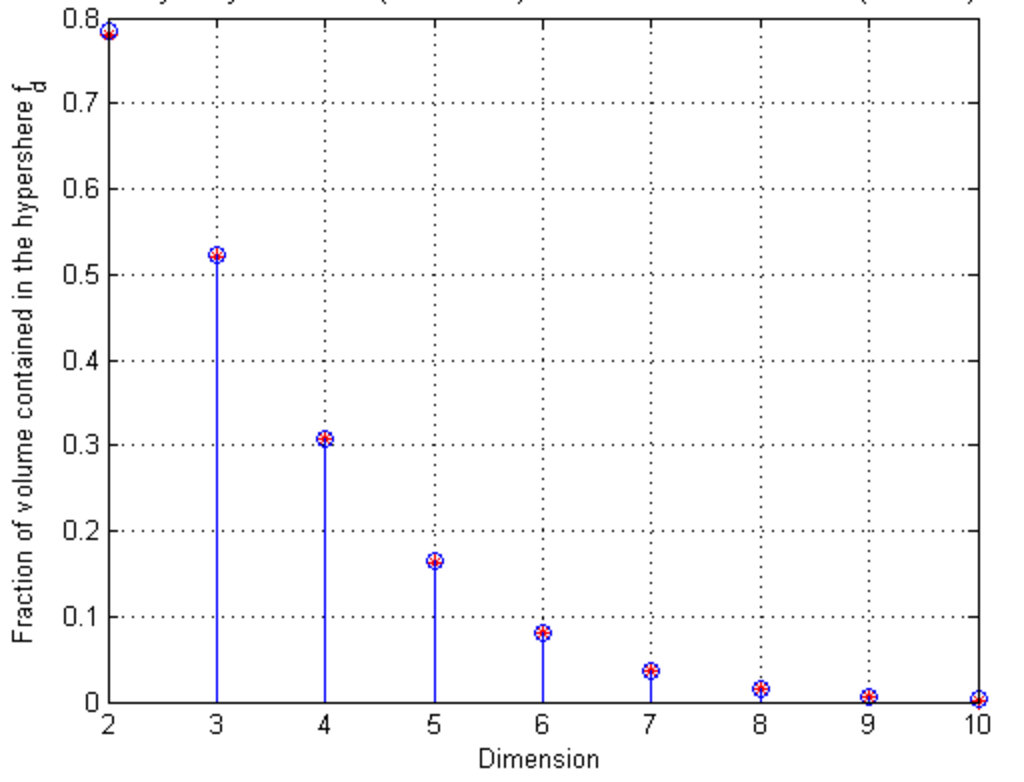
\includegraphics[scale=0.5]{prob1}
    \caption{$f_d$ vs. $d$}
    \label{fig:my_label}
\end{figure}

\newpage
\begin{problem}[Norms, Distances, and Hierarchical Clustering, 5 pts]

  Consider the following four data points, belonging to three clusters: the
  black cluster $((x_1, y_1) = (0.1, 0.5) $ and $(x_2, y_2) = (0.35, 0.75))$,
  the red cluster $(x_3, y_3) = (0.28, 1.35)$ cluster, and the blue cluster
  $(x_4, y_4) = (0, 1.01)$.

  \begin{center} 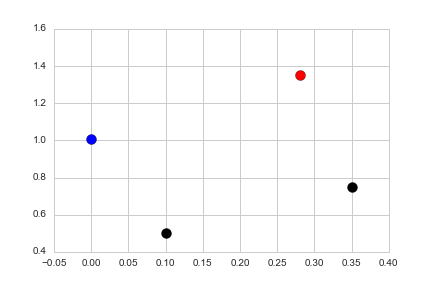
\includegraphics[scale=.4]{scatterplot.png} \end{center}
  At each step of hierarchical clustering, the two most similar (or least
  dissimilar) clusters are merged together. This step is repeated until there is
  one single group. Different distances can be used to measure group
  dissimilarity. Recall the definition of the $l_1$, $l_2$, and $l_{\infty}$
  norm:
  \begin{itemize}
    \item For $\mathbf{x} \in \mathbb{R}^n, \| \mathbf{x} \|_1 = \sum_{i = 1}^n
      |x_i|$
    \item For $\mathbf{x} \in \mathbb{R}^n, \| \mathbf{x} \|_2 = \sqrt{\sum_{i =
      1}^n x_i^2 }$
    \item For $\mathbf{x} \in \mathbb{R}^n, \| \mathbf{x} \|_{\infty} = \max_{i
      = 1}^n |x_i|$
  \end{itemize}
  Also recall the definition of single-link distance, complete-link distance,
  and average-link distance between two clusters:
  \begin{itemize}
    \item Single-link clustering: for clusters $G$ and $H$, $d_{S}(G, H) =
    \min_{i \in G, j\in H} d(i, j)$
    \item Complete-link clustering: for clusters $G$ and $H$, $d_{C}(G, H) =
    \max_{i \in G, j\in H} d(i, j)$
    \item Average-link clustering: for clusters $G$ and $H$, $d_{A}(G, H) =
      \frac{1}{|G| |H|} \sum_{i\in G}\sum_{j \in H} d(i, j)$
  \end{itemize}
  \paragraph{Warm up question.} \noindent Draw the 2D unit sphere for each norm,
  defined as $\mathcal{S} = \{x \in \mathbb{R}^2: \|x\| = 1 \}$. Feel free to do
  it by hand, take a picture and include it in your pdf.

  \paragraph{Main question.}
  \noindent For each norm ($l_1, l_2, l_\infty$) and each clustering method
  (single, complete, or average link clustering), specify which 2 clusters would
  be the first to merge.
\end{problem}
\subsection*{Solution}

\subsubsection*{Warm up question}

\begin{itemize}
\item For $\mathbf{x} \in \mathbb{R}^n, \| \mathbf{x} \|_1 = \sum_{i = 1}^n |x_i|$, see the left plot of Figure 2
\item For $\mathbf{x} \in \mathbb{R}^n, \| \mathbf{x} \|_2 = \sqrt{\sum_{i = 
1}^n x_i^2 }$, see the middle plot of Figure 2
\item For $\mathbf{x} \in \mathbb{R}^n, \| \mathbf{x} \|_{\infty} = \max_{i = 
1}^n |x_i|$, see the right plot of Figure 2
\end{itemize}

\begin{figure}[ht]
    \centering
    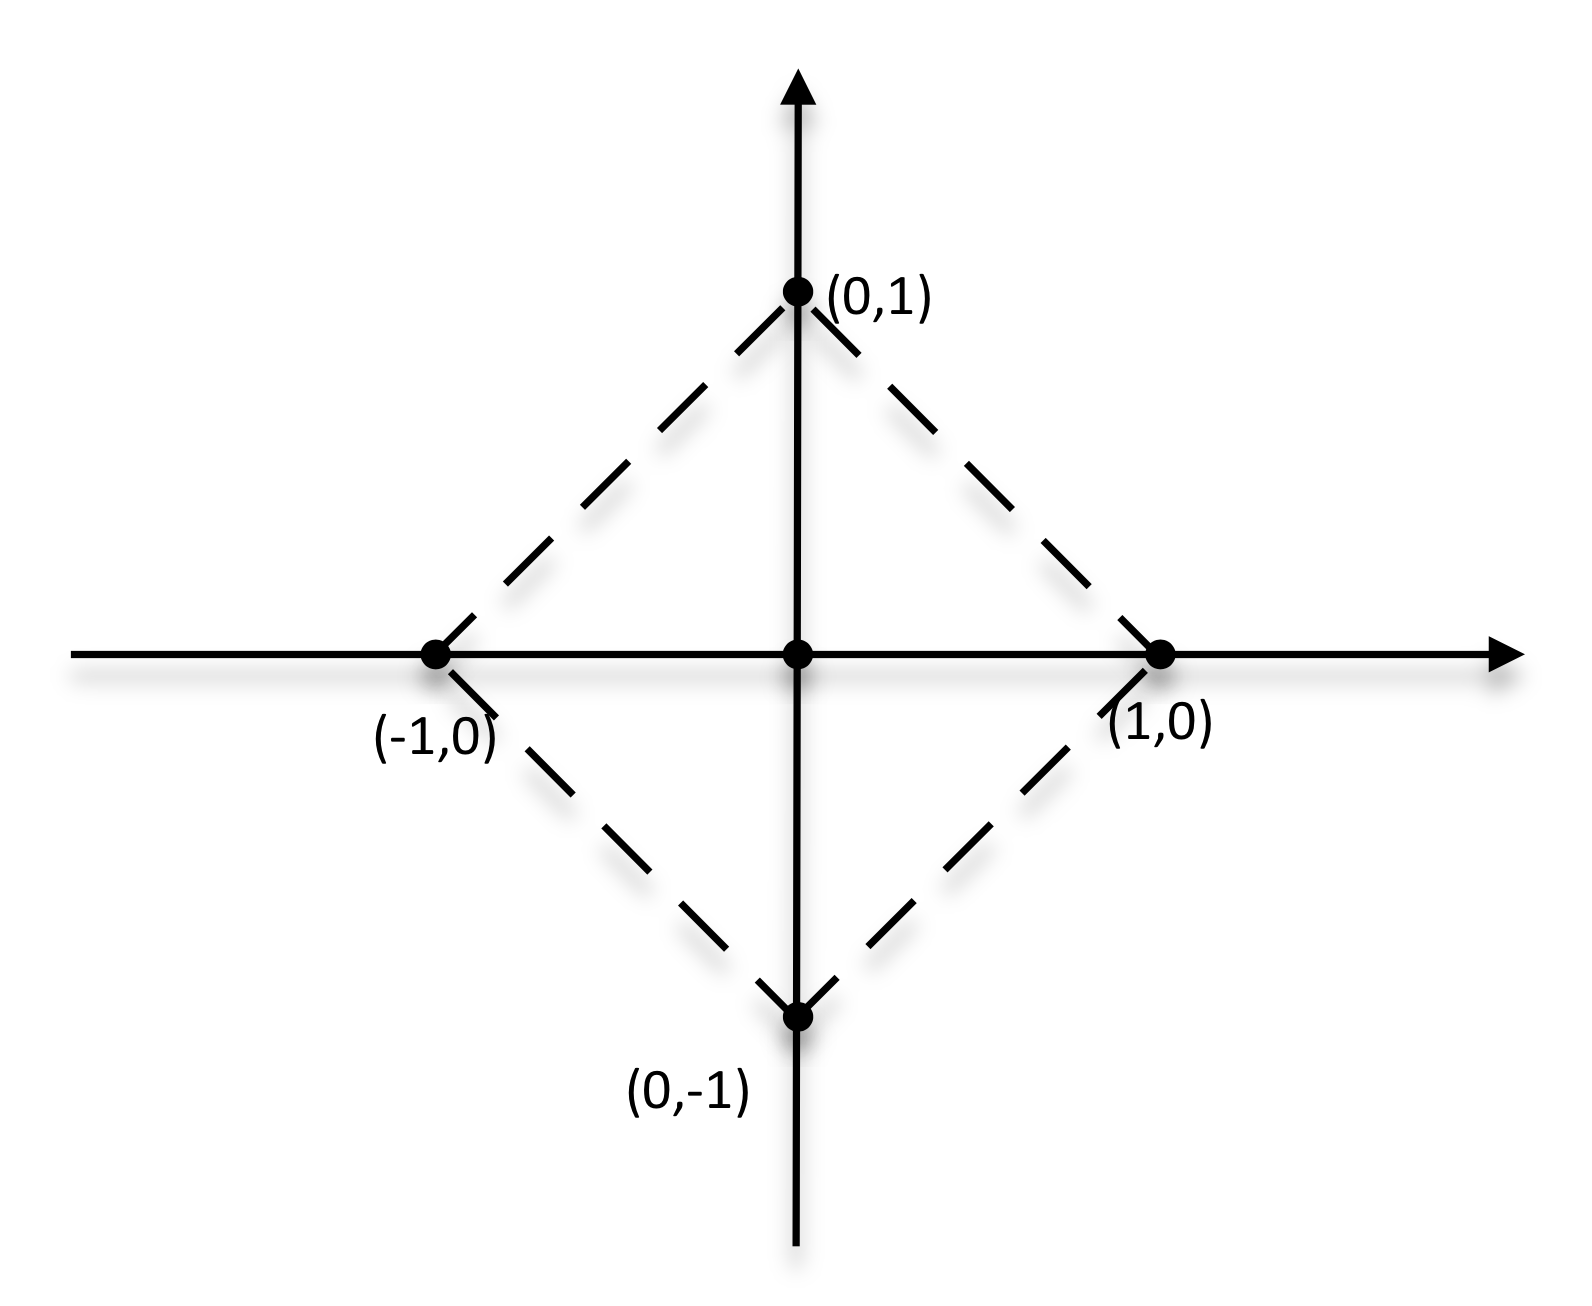
\includegraphics[scale=0.19]{prob2-1}
    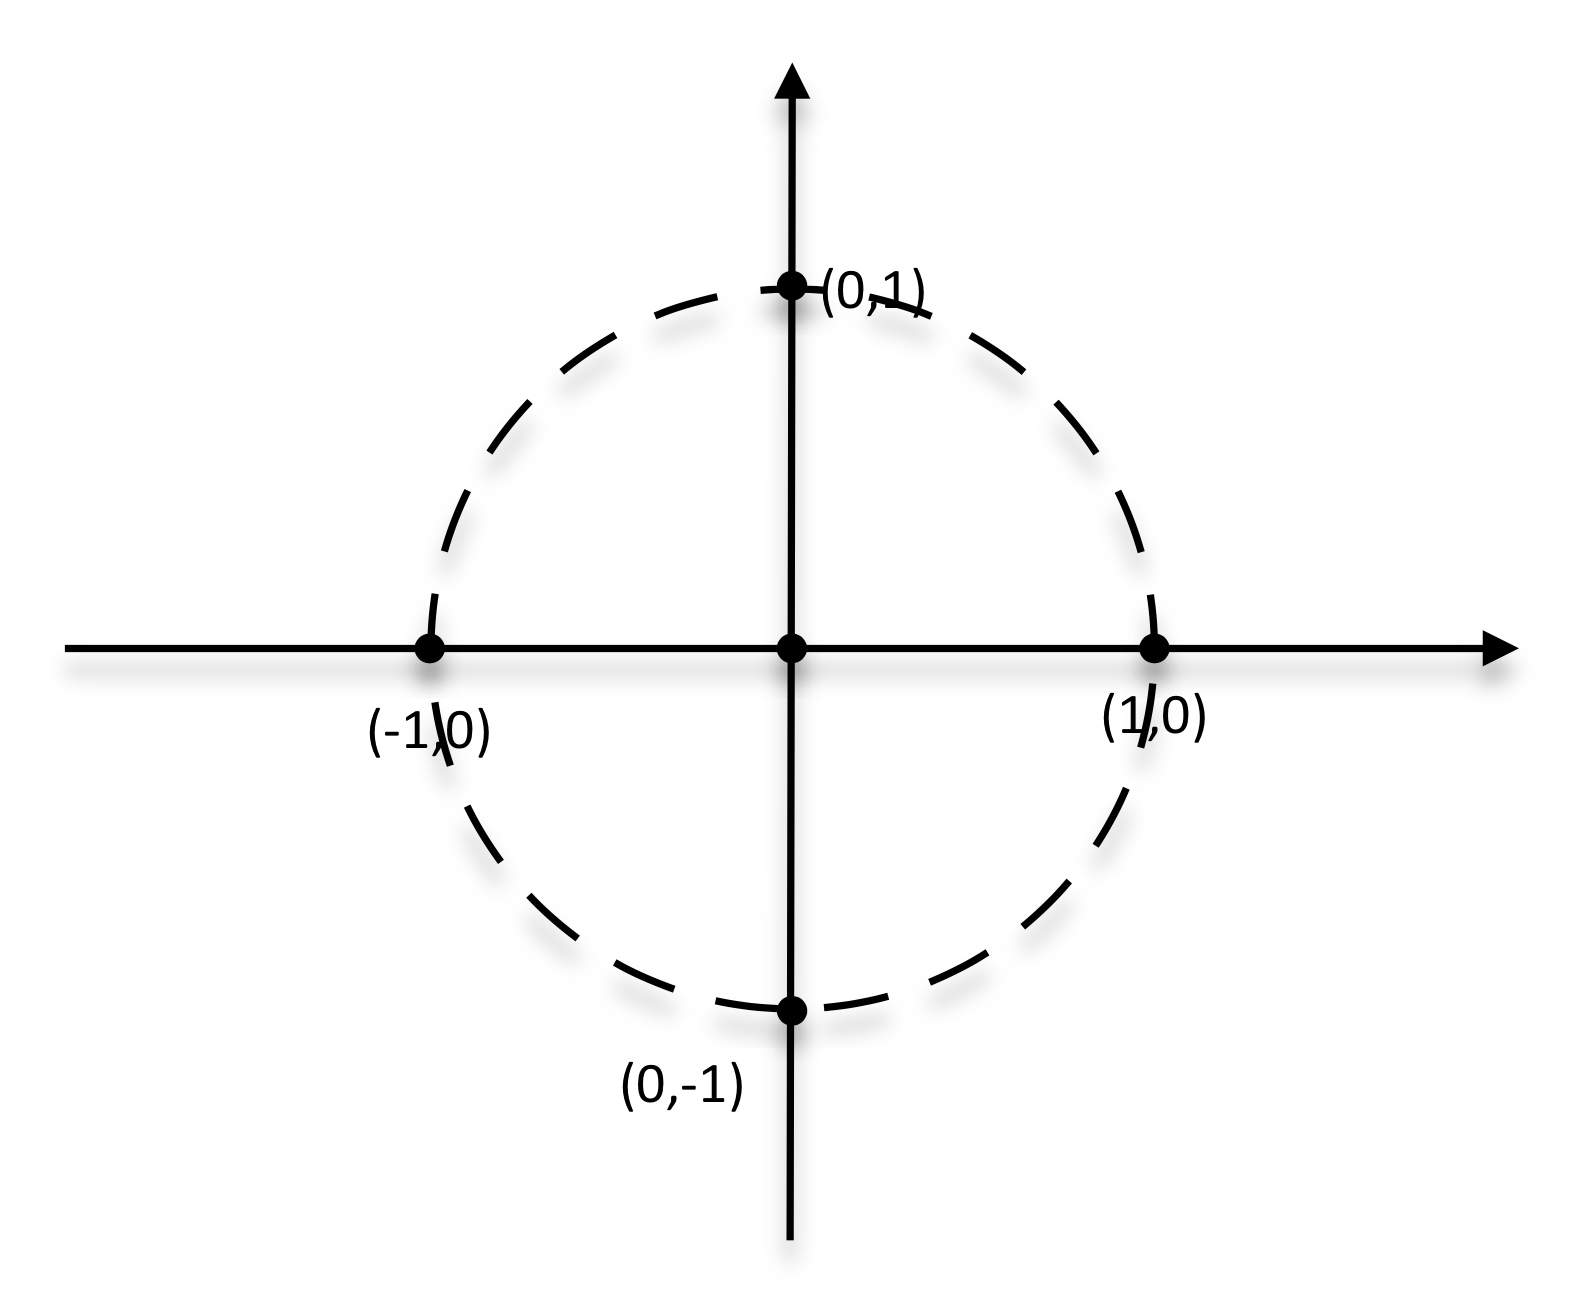
\includegraphics[scale=0.19]{prob2-2}
    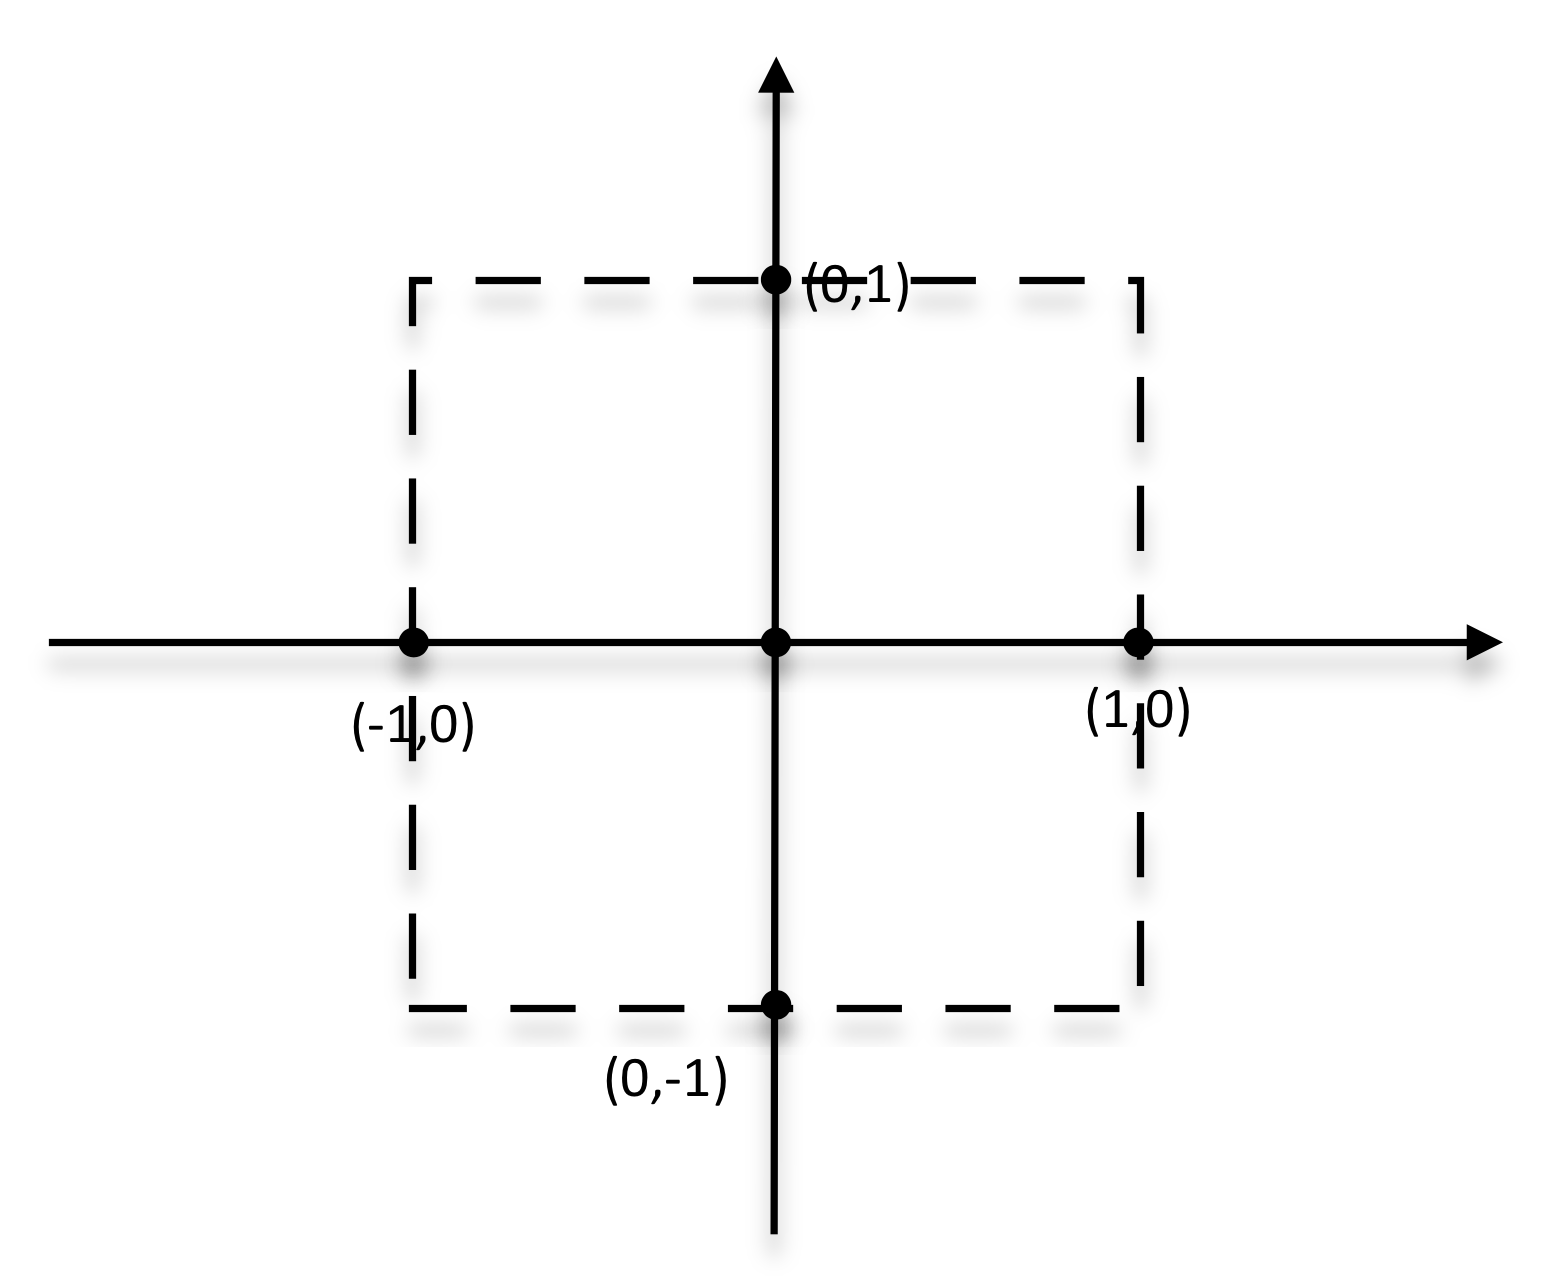
\includegraphics[scale=0.19]{prob2-3}
    \caption{2D unit sphere for three kinds of norms: $l_1, l_2, l_\infty$}
\end{figure}
    
\subsubsection*{Main question}

Denote the black, red and blue cluster as $BK$, $RD$, $BL$.

\begin{enumerate}
    \item For norm $l_1$,
    \begin{enumerate}
        \item For single-link clustering,
        \begin{align*}
            d_S(BK, RD) &= \min_{i\in BK, j\in RD}d(i,j) = d(2,3) = 0.67 \\
            d_S(BK, BL) &= \min_{i\in BK, j\in BL}d(i,j) = d(1,4) = d(2,4) = 0.61 \\
            d_S(RD, BL) &= \min_{i\in RD, j\in BL}d(i,j) = d(3,4) = 0.62
        \end{align*}
        therefore the black cluster and the blue cluster would be the first to merge.
        
        \item For complete-link clustering,
        \begin{align*}
            d_C(BK, RD) &= \max_{i\in BK, j\in RD}d(i,j) = d(1,3) = 1.03 \\
            d_C(BK, BL) &= \max_{i\in BK, j\in BL}d(i,j) = d(1,4) = d(2,4) = 0.61 \\
            d_C(RD, BL) &= \max_{i\in RD, j\in BL}d(i,j) = d(3,4) = 0.62
        \end{align*}
        therefore the black cluster and the blue cluster would be the first to merge.
        
        \item For average-link clustering,
        \begin{align*}
            d_A(BK, RD) &= \text{avg}_{i\in BK, j\in RD}d(i,j) = \frac{d(1,3) + d(2,3)}{2} = 0.85 \\
            d_A(BK, BL) &= \text{avg}_{i\in BK, j\in BL}d(i,j) = \frac{d(1,4) + d(2,4)}{2} = 0.61 \\
            d_A(RD, BL) &= \text{avg}_{i\in RD, j\in BL}d(i,j) = d(3,4) = 0.62
        \end{align*}
        therefore the black cluster and the blue cluster would be the first to merge.
    \end{enumerate}
    
    \item For norm $l_2$,
    \begin{enumerate}
        \item For single-link clustering,
        \begin{align*}
            d_S(BK, RD) &= \min_{i\in BK, j\in RD}d(i,j) = d(2,3) = 0.604 \\
            d_S(BK, BL) &= \min_{i\in BK, j\in BL}d(i,j) = d(2,4) = 0.436 \\
            d_S(RD, BL) &= \min_{i\in RD, j\in BL}d(i,j) = d(3,4) = 0.440
        \end{align*}
        therefore the black cluster and the blue cluster would be the first to merge.
        
        \item For complete-link clustering,
        \begin{align*}
            d_C(BK, RD) &= \max_{i\in BK, j\in RD}d(i,j) = d(1,3) = 0.869 \\
            d_C(BK, BL) &= \max_{i\in BK, j\in BL}d(i,j) = d(1,4) = 0.520 \\
            d_C(RD, BL) &= \max_{i\in RD, j\in BL}d(i,j) = d(3,4) = 0.440
        \end{align*}
        therefore the red cluster and the blue cluster would be the first to merge.
        
        \item For average-link clustering,
        \begin{align*}
            d_A(BK, RD) &= \text{avg}_{i\in BK, j\in RD}d(i,j) = \frac{d(1,3) + d(2,3)}{2} = 0.736 \\
            d_A(BK, BL) &= \text{avg}_{i\in BK, j\in BL}d(i,j) = \frac{d(1,4) + d(2,4)}{2} = 0.478 \\
            d_A(RD, BL) &= \text{avg}_{i\in RD, j\in BL}d(i,j) = d(3,4) = 0.440
        \end{align*}
        therefore the red cluster and the blue cluster would be the first to merge.
    \end{enumerate}
    
    \item For norm $l_3$,
    \begin{enumerate}
        \item For single-link clustering,
        \begin{align*}
            d_S(BK, RD) &= \min_{i\in BK, j\in RD}d(i,j) = d(2,3) = 0.60 \\
            d_S(BK, BL) &= \min_{i\in BK, j\in BL}d(i,j) = d(2,4) = 0.35 \\
            d_S(RD, BL) &= \min_{i\in RD, j\in BL}d(i,j) = d(3,4) = 0.34
        \end{align*}
        therefore the red cluster and the blue cluster would be the first to merge.
        
        \item For complete-link clustering,
        \begin{align*}
            d_C(BK, RD) &= \max_{i\in BK, j\in RD}d(i,j) = d(1,3) = 0.85 \\
            d_C(BK, BL) &= \max_{i\in BK, j\in BL}d(i,j) = d(1,4) = 0.51 \\
            d_C(RD, BL) &= \max_{i\in RD, j\in BL}d(i,j) = d(3,4) = 0.34
        \end{align*}
        therefore the red cluster and the blue cluster would be the first to merge.
        
        \item For average-link clustering,
        \begin{align*}
            d_A(BK, RD) &= \text{avg}_{i\in BK, j\in RD}d(i,j) = \frac{d(1,3) + d(2,3)}{2} = 0.725 \\
            d_A(BK, BL) &= \text{avg}_{i\in BK, j\in BL}d(i,j) = \frac{d(1,4) + d(2,4)}{2} = 0.43 \\
            d_A(RD, BL) &= \text{avg}_{i\in RD, j\in BL}d(i,j) = d(3,4) = 0.34
        \end{align*}
        therefore the red cluster and the blue cluster would be the first to merge.
    \end{enumerate}
\end{enumerate}
    
\newpage

\section*{K-Means [15 pts]}
Implement K-Means clustering from scratch.\footnote{That is, don't use a
third-party machine learning implementation like \texttt{scikit-learn};
\texttt{numpy} is fine.}. You have been provided with the MNIST dataset. You can
learn more about it at  \url{http://yann.lecun.com/exdb/mnist/}. The MNIST task
is widely used in supervised learning, and modern algorithms with neural
networks do very well on this task. We can also use MNIST for interesting
unsupervised tasks. You are given representations of 6000 MNIST images, each of
which are $28\times28$  handwritten digits. In this problem, you will implement
K-means clustering on MNIST, to show how this relatively simple algorithm can
cluster similar-looking images together quite well.

\begin{problem}[K-means, 15pts]
The given code loads the images into your environment as a 6000x28x28 array.
Implement K-means clustering on it for a few different values of $K$, and show
results from the fit. Show the mean images for each class, and by selecting a
few representative images for each class. You should explain how you selected
these representative images. To render an image, use the numpy imshow function,
which the distribution code gives an example of. Use squared norm as your
distance metric. You should feel free to explore other metrics along with
squared norm if you are interested in seeing the effects of using those. Also,
your code should use the entire provided 6000-image dataset (which, by the way,
is only 10\% of the full MNIST set).

Are the results wildly different for different restarts and/or different $K$?
Plot the K-means objective function as a function of iteration and verify that
it never increases.

Finally, implement K-means++ and see if gives you more satisfying
initializations (and final results) for K-means. Explain your findings.

As in past problem sets, please include your plots in this document. There may
be tons of plots for this problem, so feel free to take up multiple pages, as
long as it is organized.
\end{problem}
\subsection*{Solution}

\subsubsection*{Implementation and results}

Implementations can be found at link \url{https://github.com/harvard-ml-courses/cs181-s16-homework1-weiyialanchen/tree/master/homework4}, and the results of $K=10$ from the fit is shown via mean images for each class, and by selecting a few representative images for each class (below are the mean images with 3 representative images right after each mean image for each class, Figure 3 - 12) - 

\begin{figure}[ht]
    \centering
    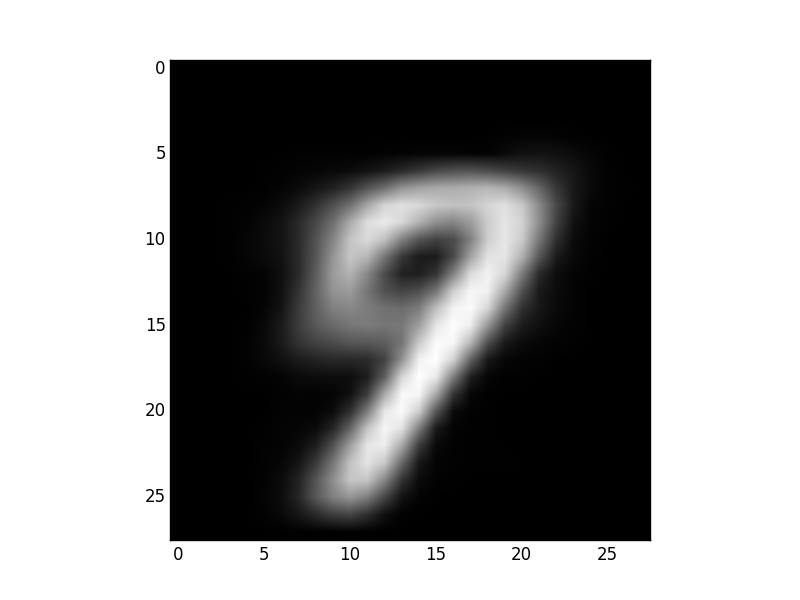
\includegraphics[scale=0.20]{mean-0}
    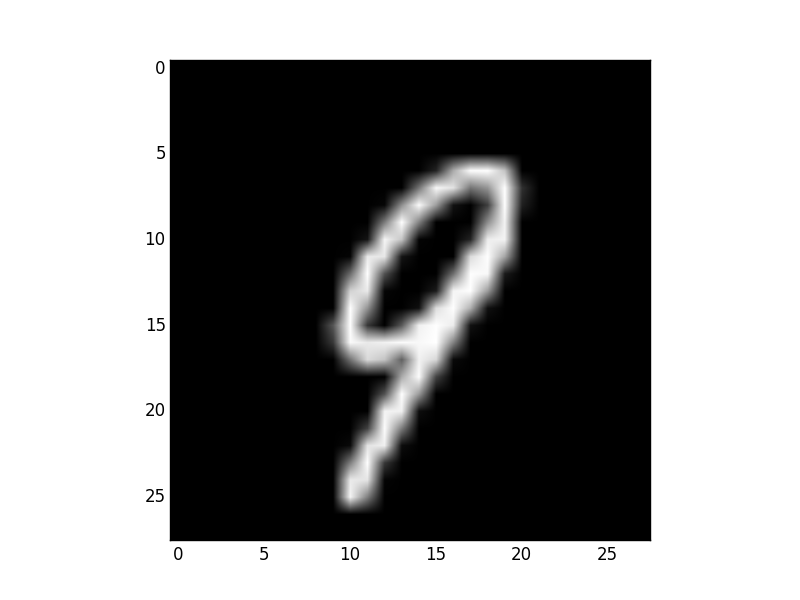
\includegraphics[scale=0.20]{representative-0-0}
    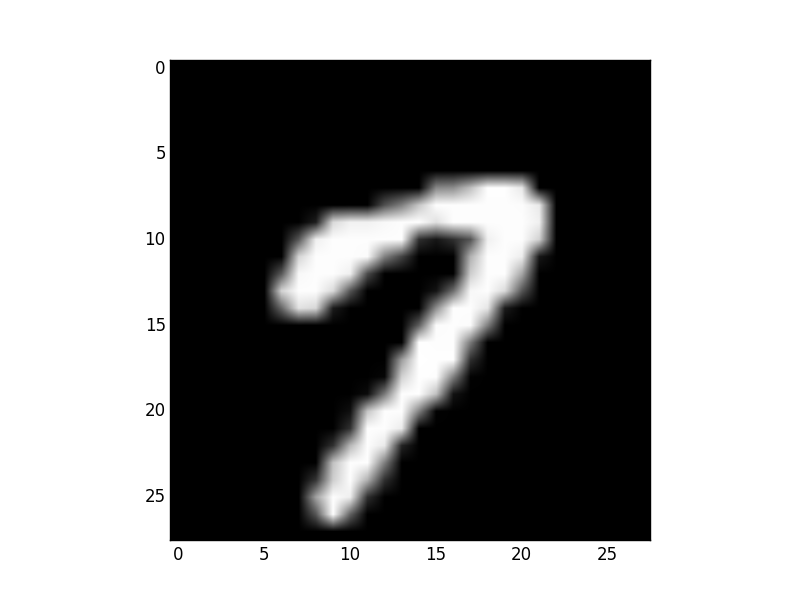
\includegraphics[scale=0.20]{representative-0-1}
    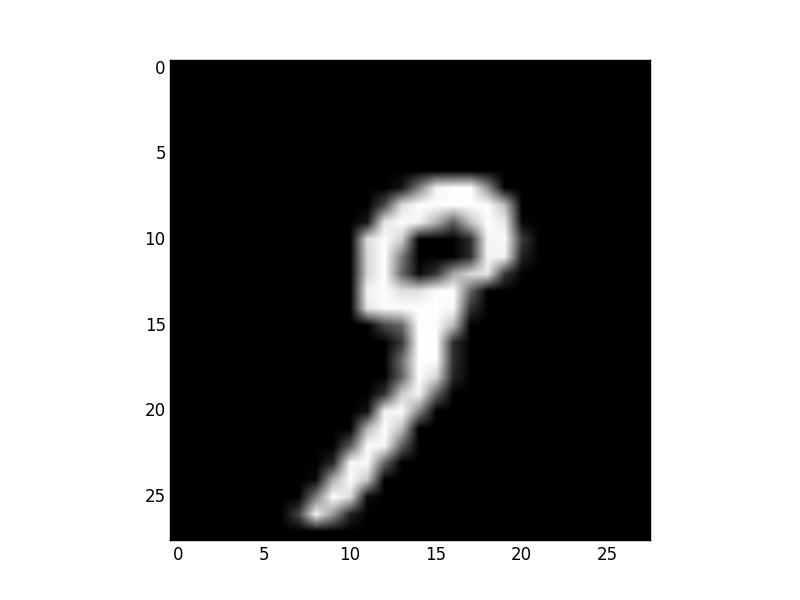
\includegraphics[scale=0.20]{representative-0-2}
    \caption{Class 1 for $K=10$}
\end{figure}

\begin{figure}[ht]
    \centering
    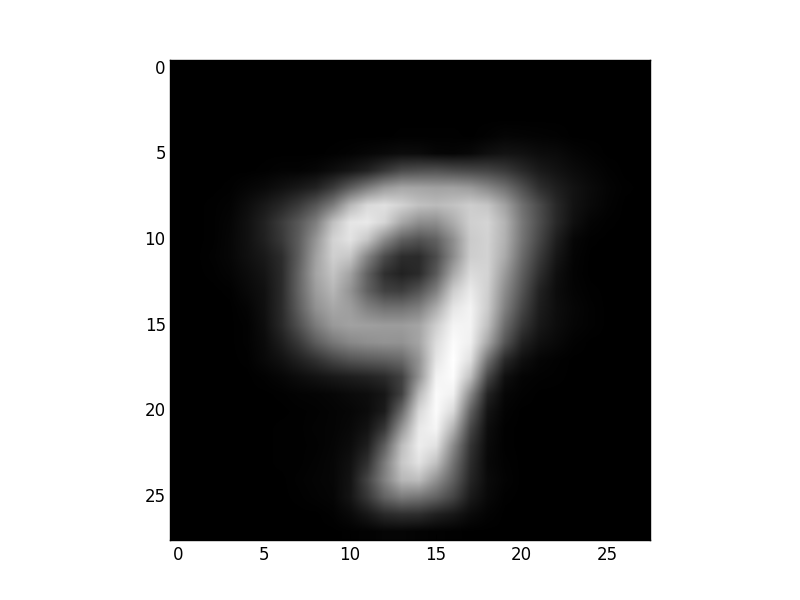
\includegraphics[scale=0.20]{mean-1}
    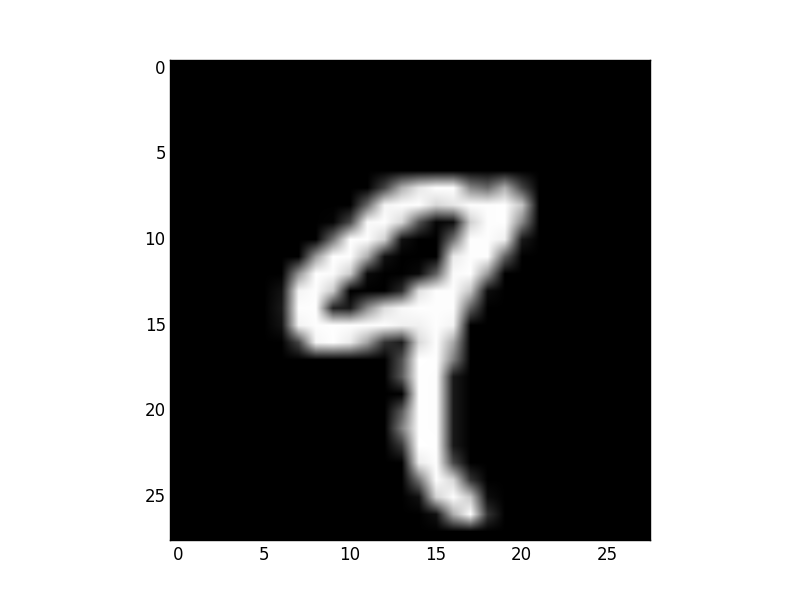
\includegraphics[scale=0.20]{representative-1-0}
    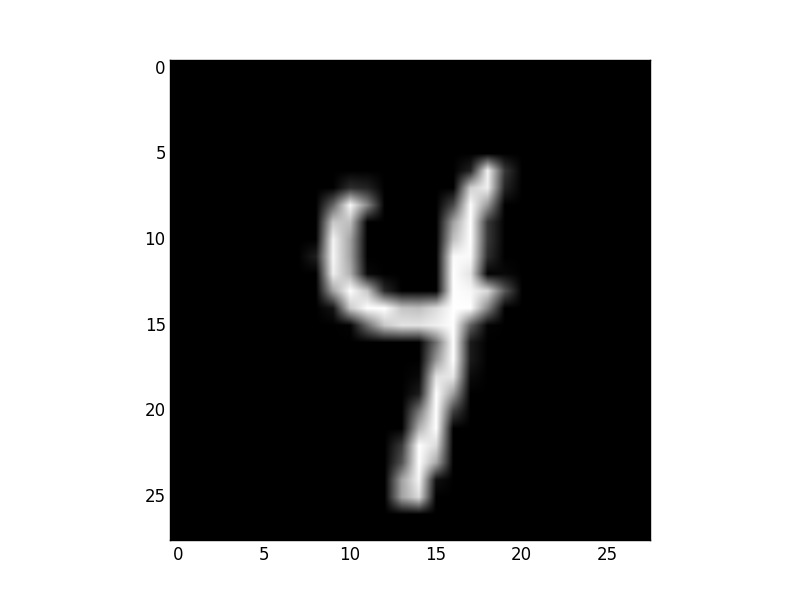
\includegraphics[scale=0.20]{representative-1-1}
    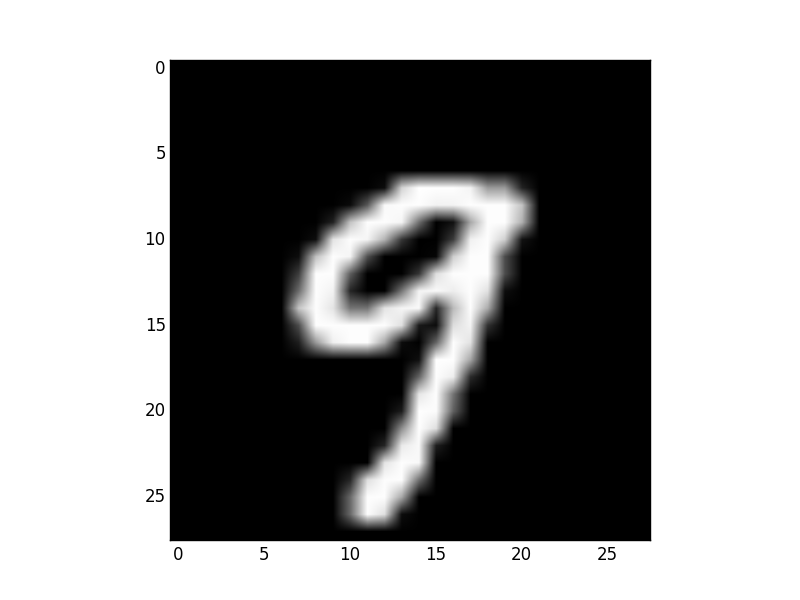
\includegraphics[scale=0.20]{representative-1-2}
    \caption{Class 2 for $K=10$}
\end{figure}

\begin{figure}[ht]
    \centering
    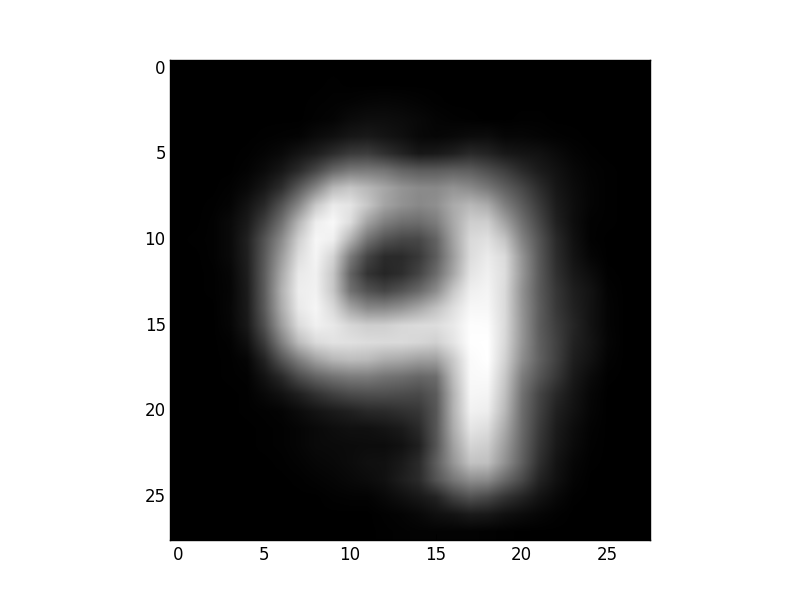
\includegraphics[scale=0.20]{mean-2}
    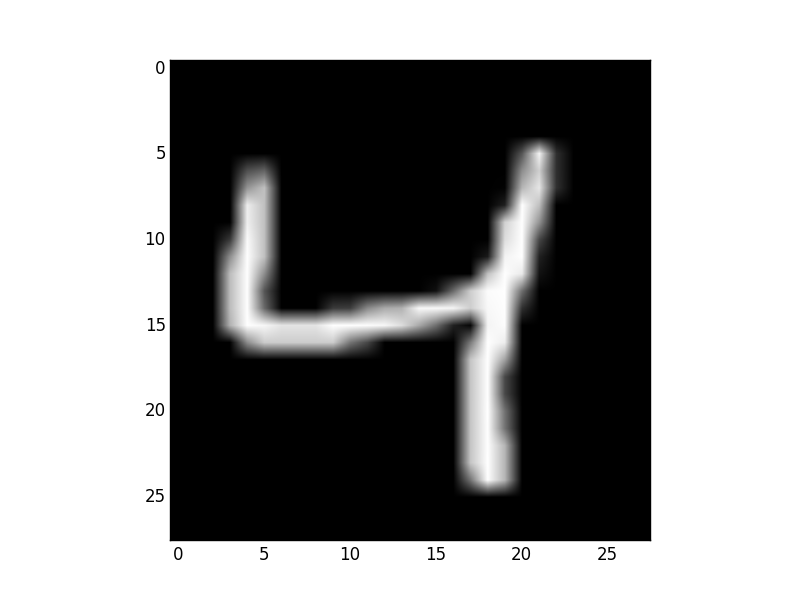
\includegraphics[scale=0.20]{representative-2-0}
    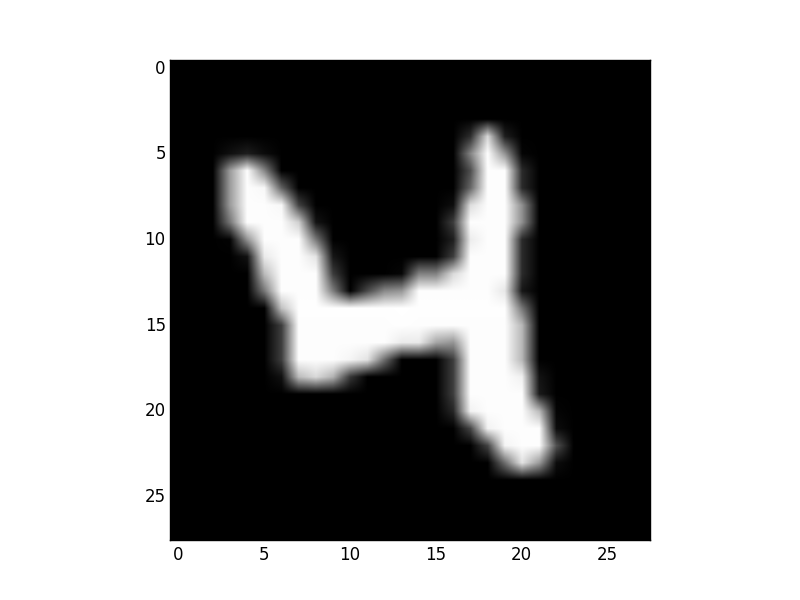
\includegraphics[scale=0.20]{representative-2-1}
    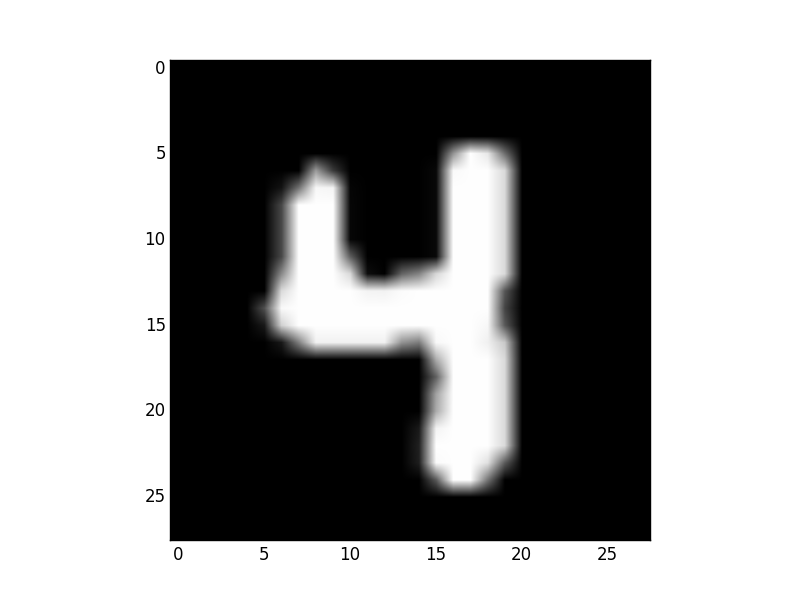
\includegraphics[scale=0.20]{representative-2-2}
    \caption{Class 3 for $K=10$}
\end{figure}

\begin{figure}[ht]
    \centering
    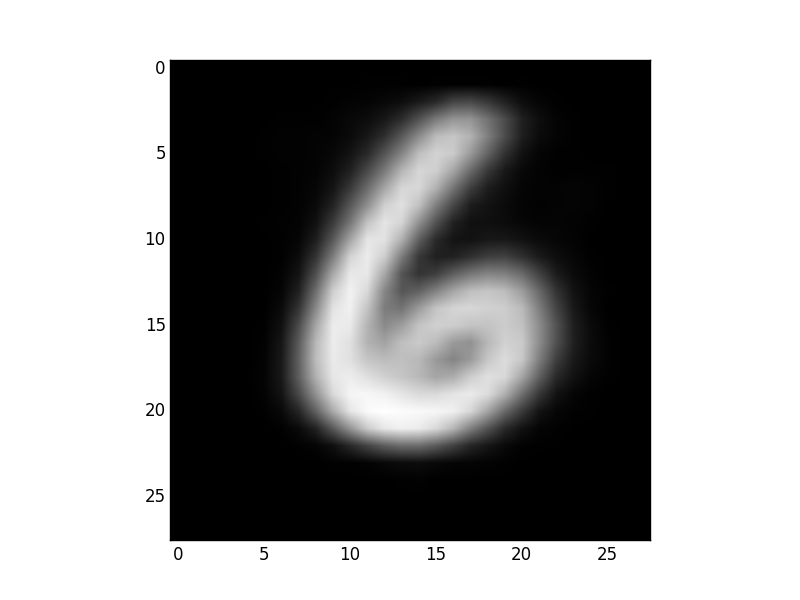
\includegraphics[scale=0.20]{mean-3}
    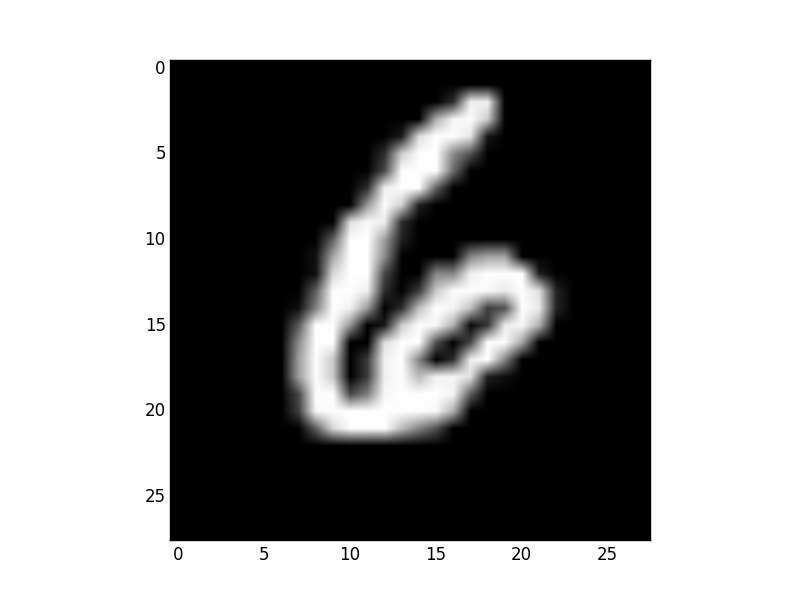
\includegraphics[scale=0.20]{representative-3-0}
    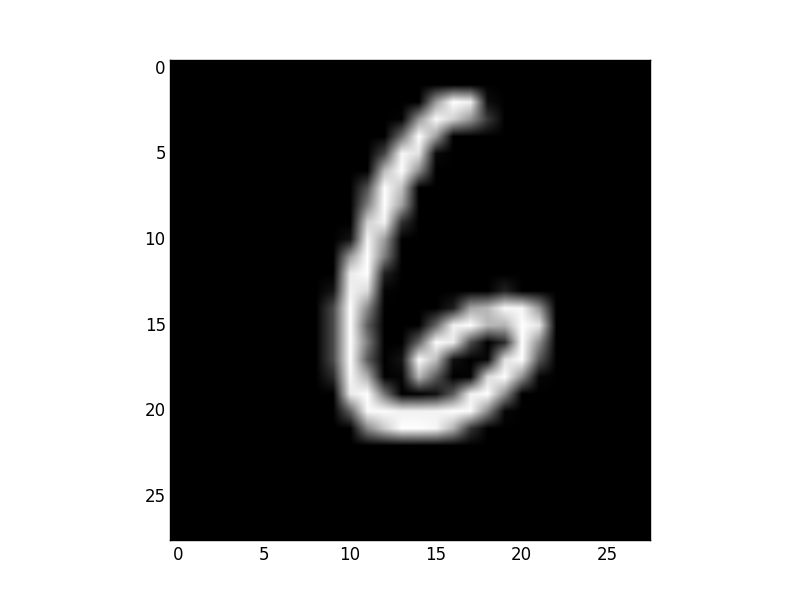
\includegraphics[scale=0.20]{representative-3-1}
    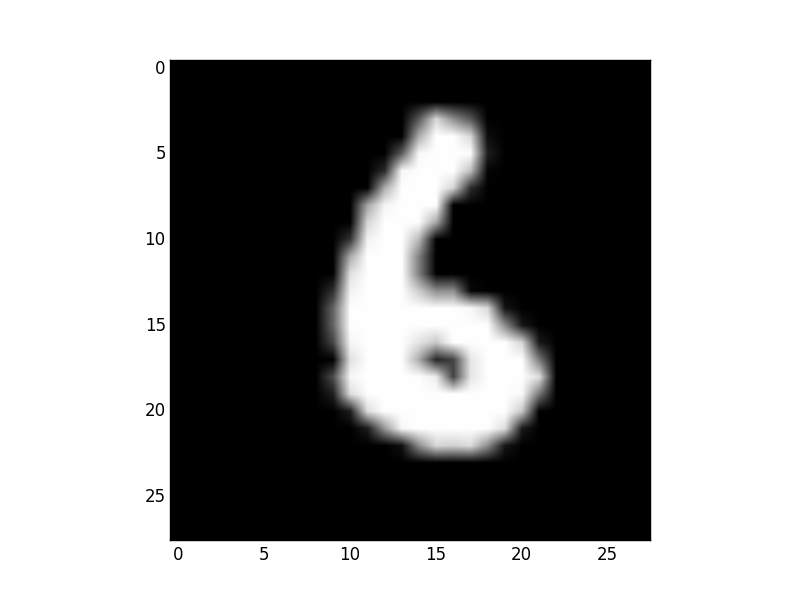
\includegraphics[scale=0.20]{representative-3-2}
    \caption{Class 4 for $K=10$}
\end{figure}

\begin{figure}[ht]
    \centering
    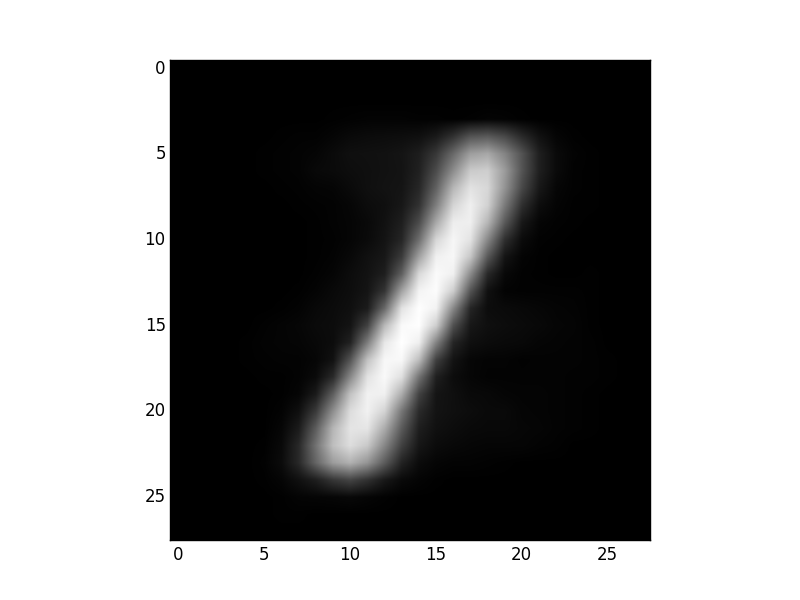
\includegraphics[scale=0.20]{mean-4}
    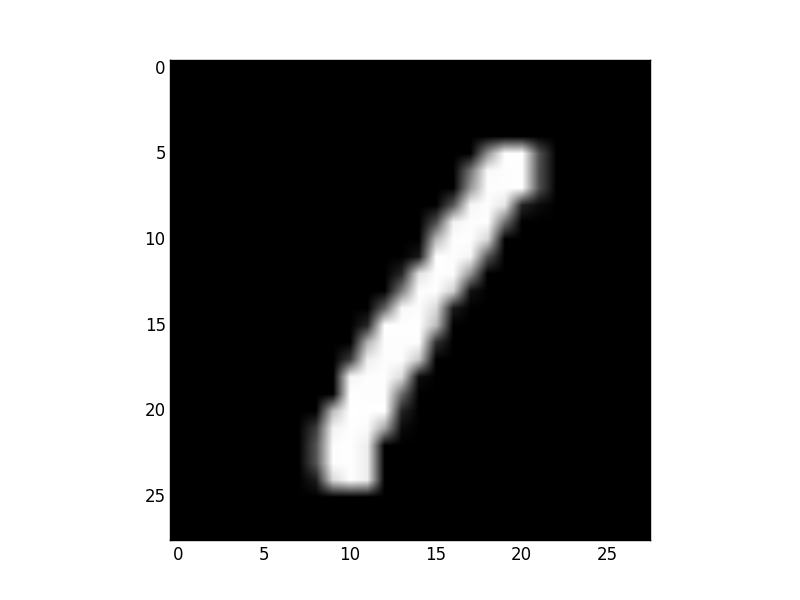
\includegraphics[scale=0.20]{representative-4-0}
    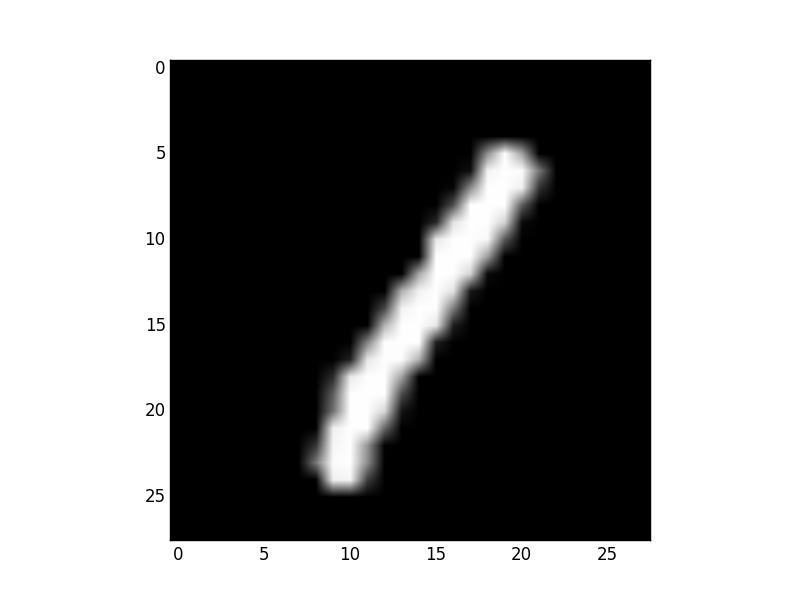
\includegraphics[scale=0.20]{representative-4-1}
    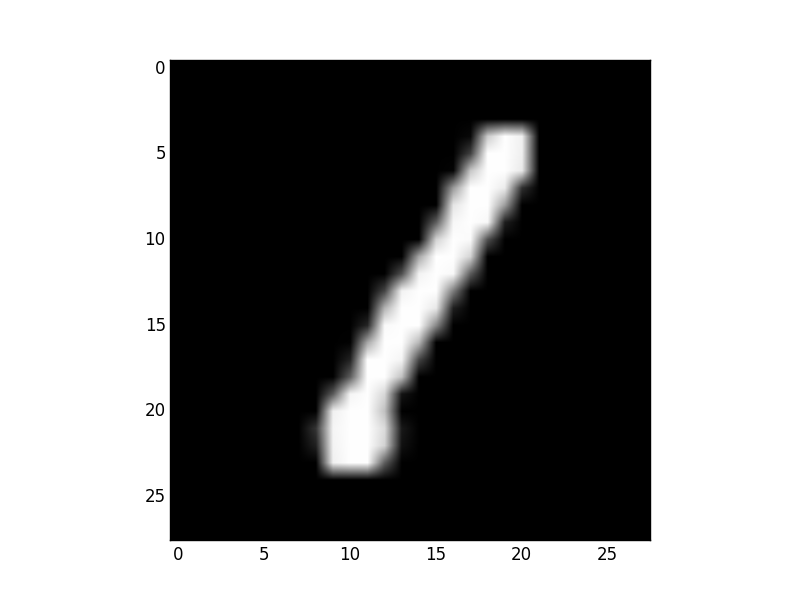
\includegraphics[scale=0.20]{representative-4-2}
    \caption{Class 5 for $K=10$}
\end{figure}

\begin{figure}[ht]
    \centering
    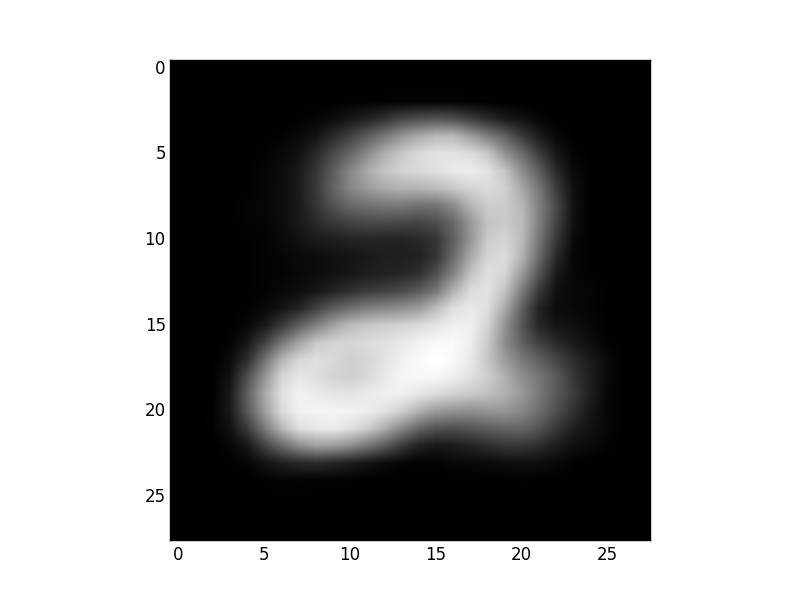
\includegraphics[scale=0.20]{mean-5}
    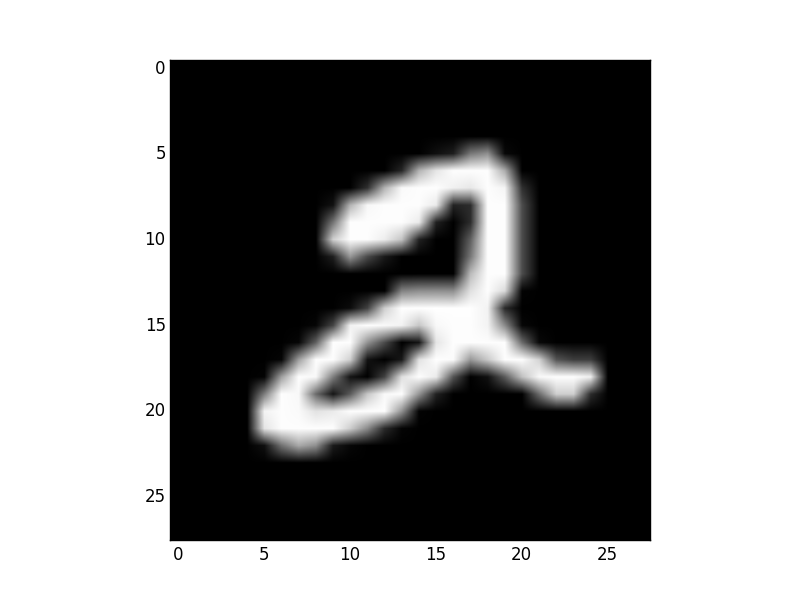
\includegraphics[scale=0.20]{representative-5-0}
    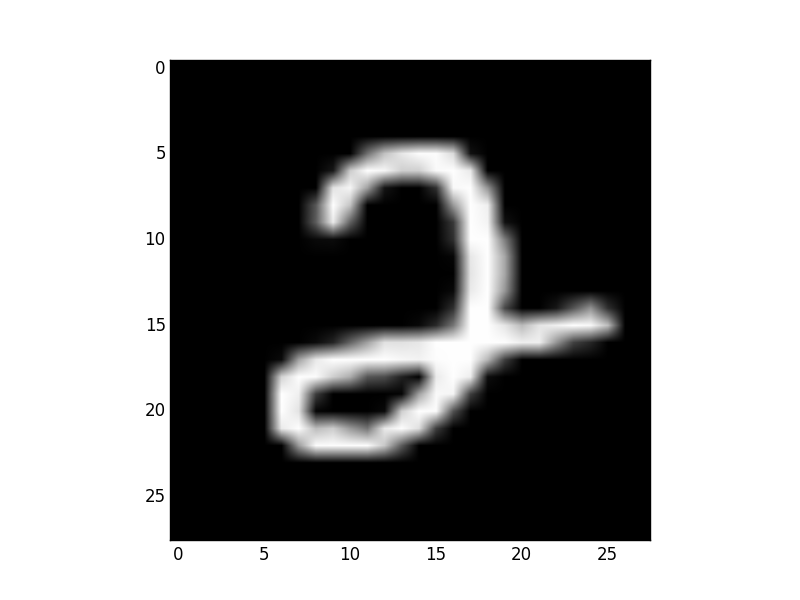
\includegraphics[scale=0.20]{representative-5-1}
    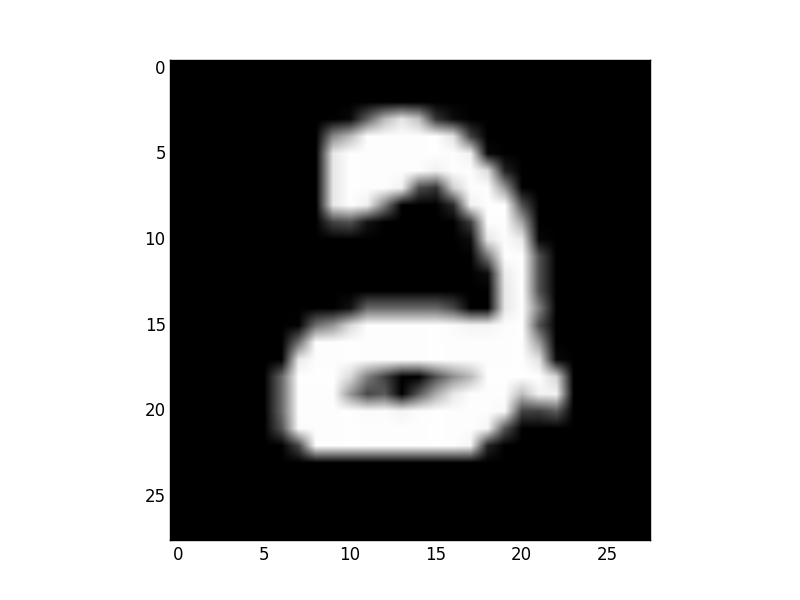
\includegraphics[scale=0.20]{representative-5-2}
    \caption{Class 6 for $K=10$}
\end{figure}

\begin{figure}[ht]
    \centering
    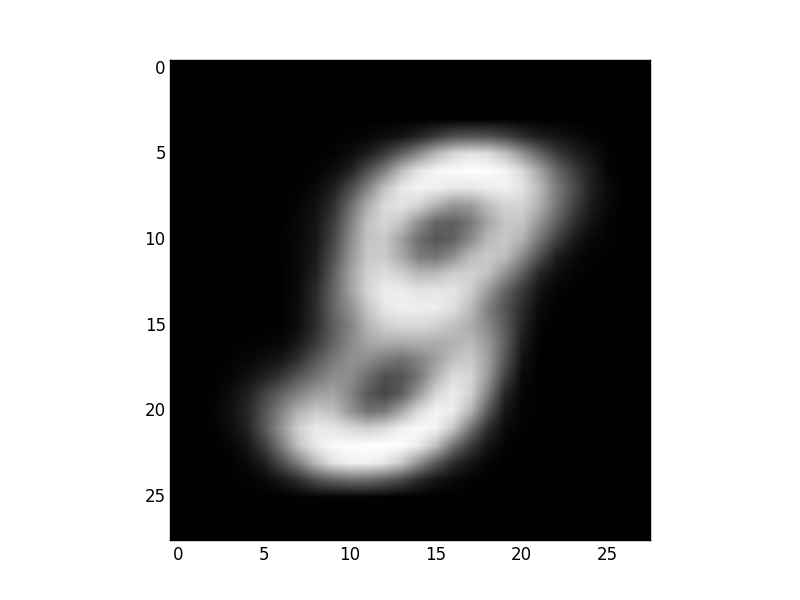
\includegraphics[scale=0.20]{mean-6}
    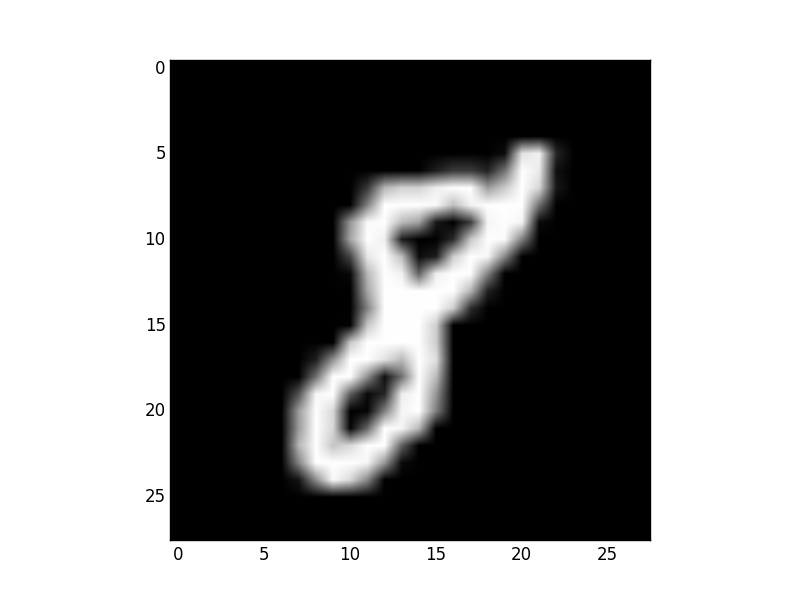
\includegraphics[scale=0.20]{representative-6-0}
    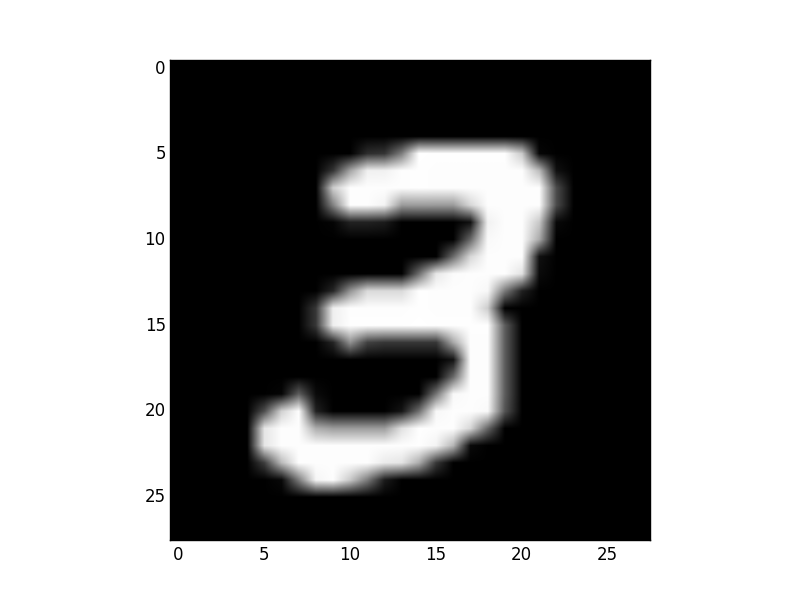
\includegraphics[scale=0.20]{representative-6-1}
    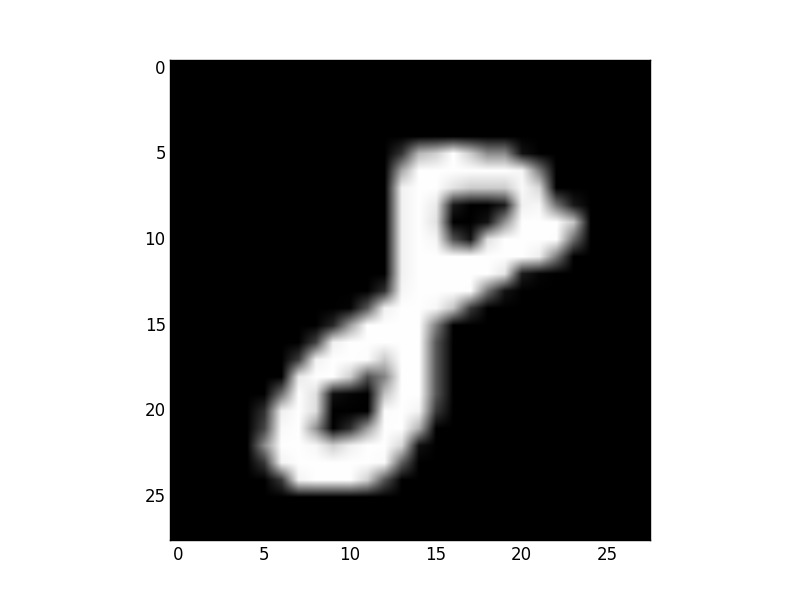
\includegraphics[scale=0.20]{representative-6-2}
    \caption{Class 7 for $K=10$}
\end{figure}

\begin{figure}[ht]
    \centering
    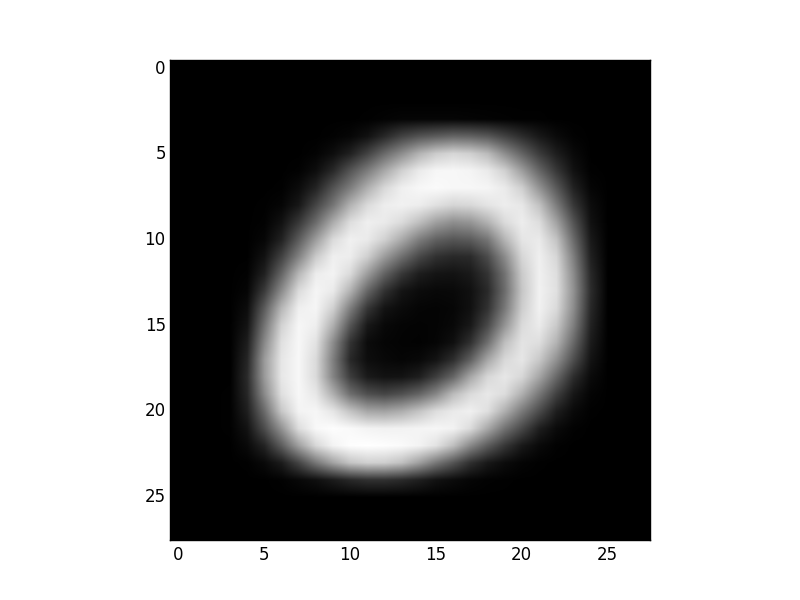
\includegraphics[scale=0.20]{mean-7}
    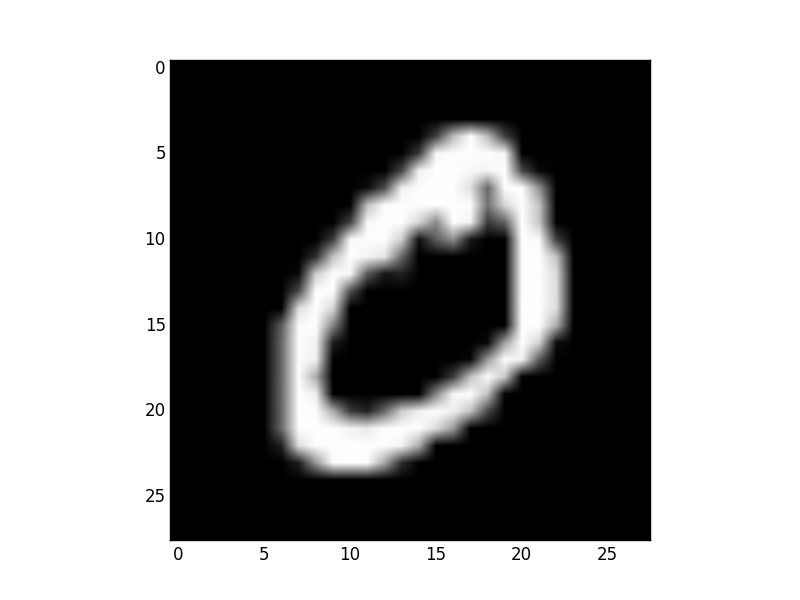
\includegraphics[scale=0.20]{representative-7-0}
    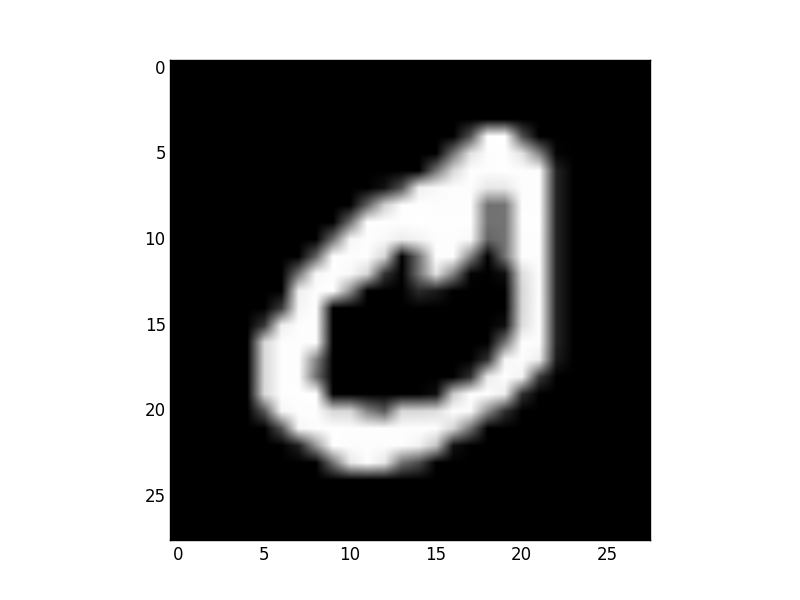
\includegraphics[scale=0.20]{representative-7-1}
    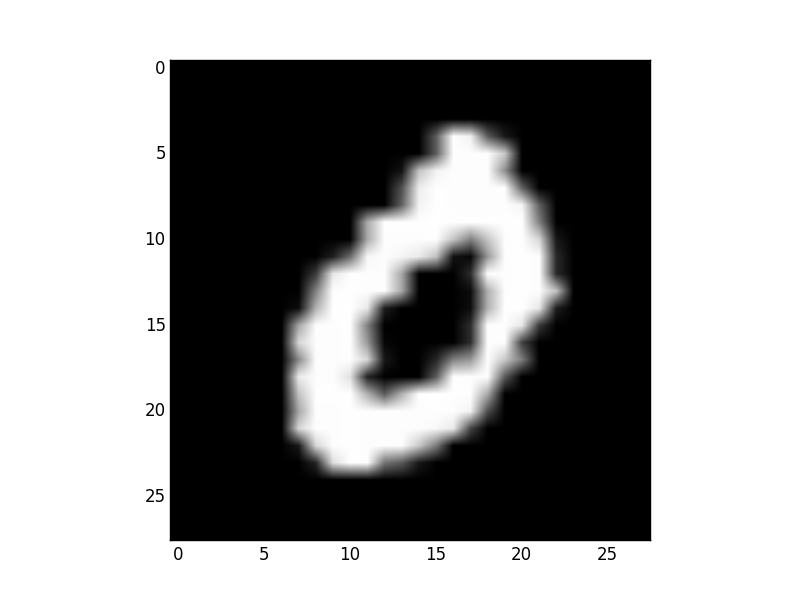
\includegraphics[scale=0.20]{representative-7-2}
    \caption{Class 8 for $K=10$}
\end{figure}

\begin{figure}[ht]
    \centering
    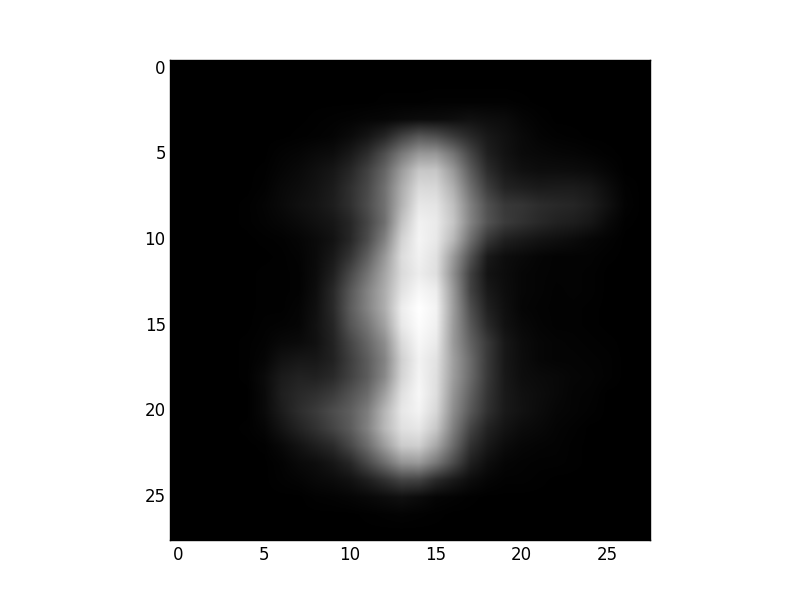
\includegraphics[scale=0.20]{mean-8}
    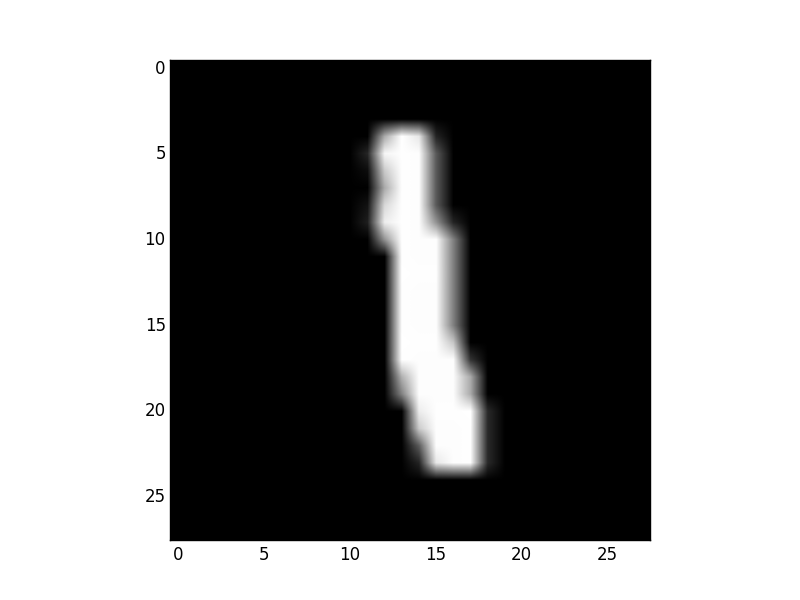
\includegraphics[scale=0.20]{representative-8-0}
    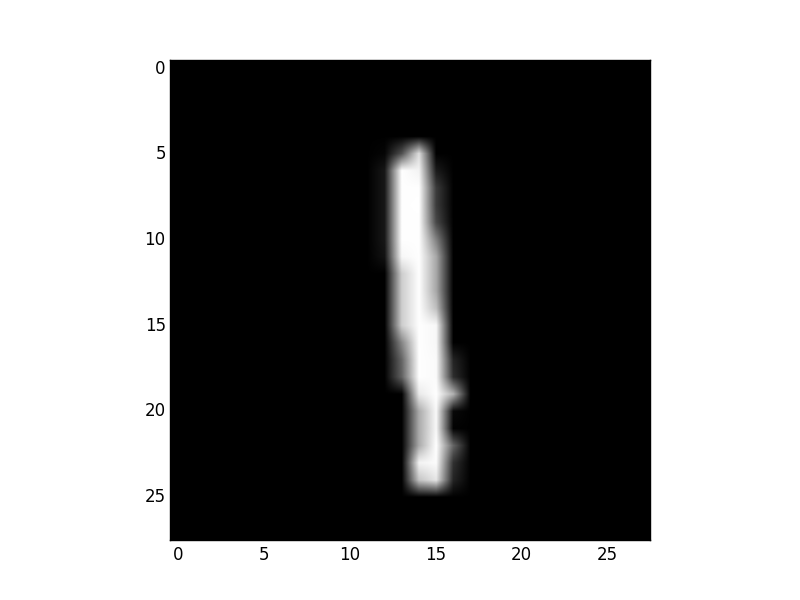
\includegraphics[scale=0.20]{representative-8-1}
    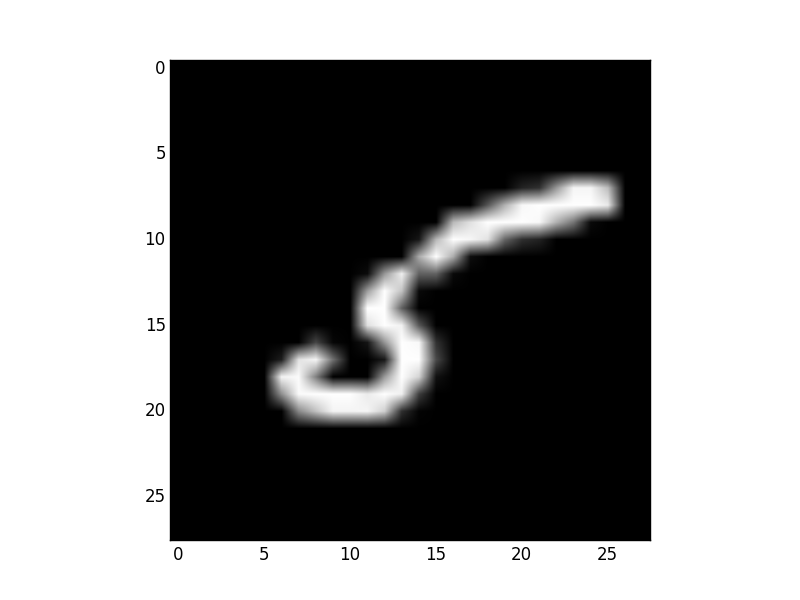
\includegraphics[scale=0.20]{representative-8-2}
    \caption{Class 9 for $K=10$}
\end{figure}

\begin{figure}[ht]
    \centering
    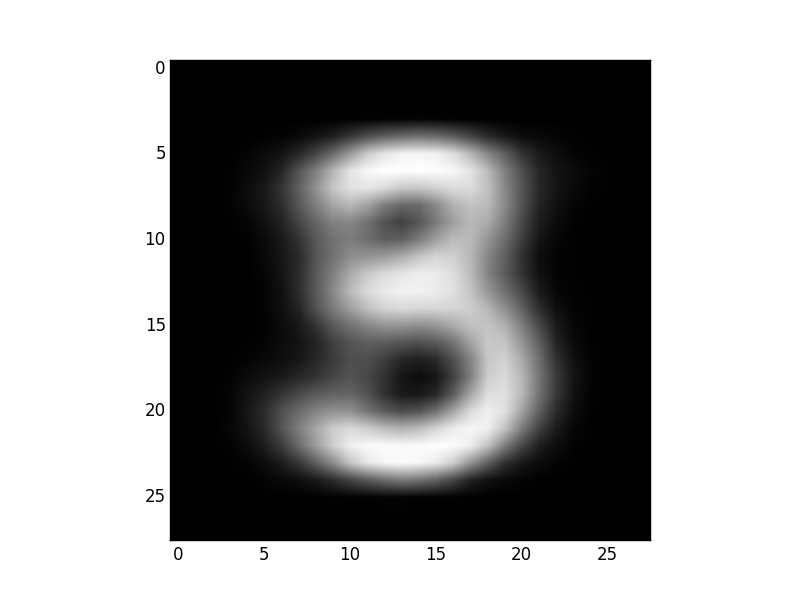
\includegraphics[scale=0.20]{mean-9}
    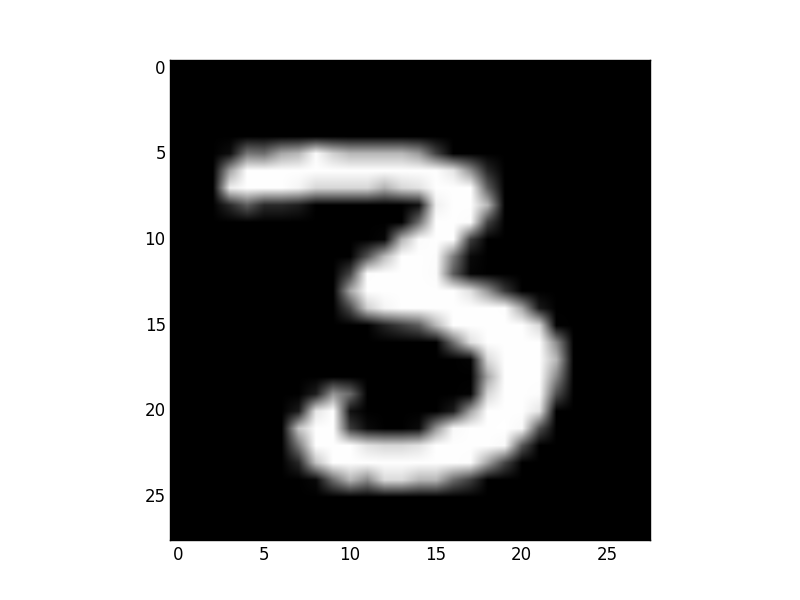
\includegraphics[scale=0.20]{representative-9-0}
    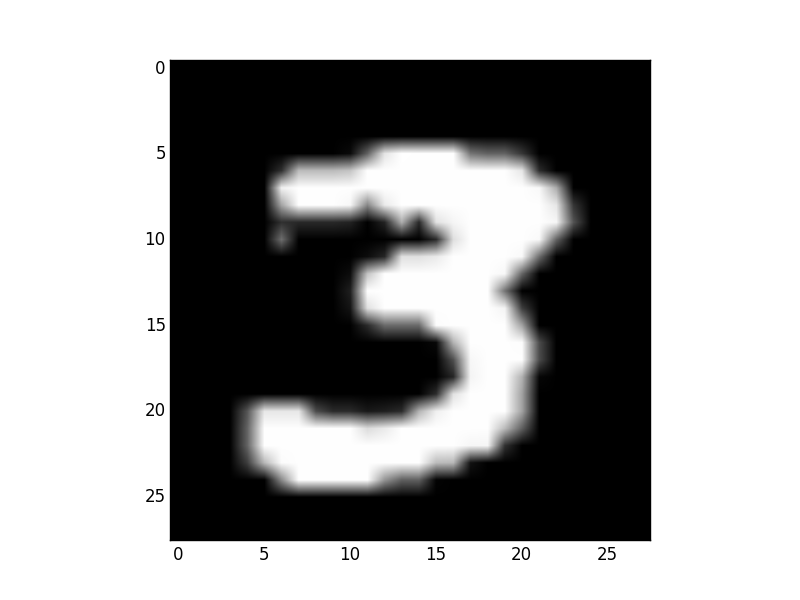
\includegraphics[scale=0.20]{representative-9-1}
    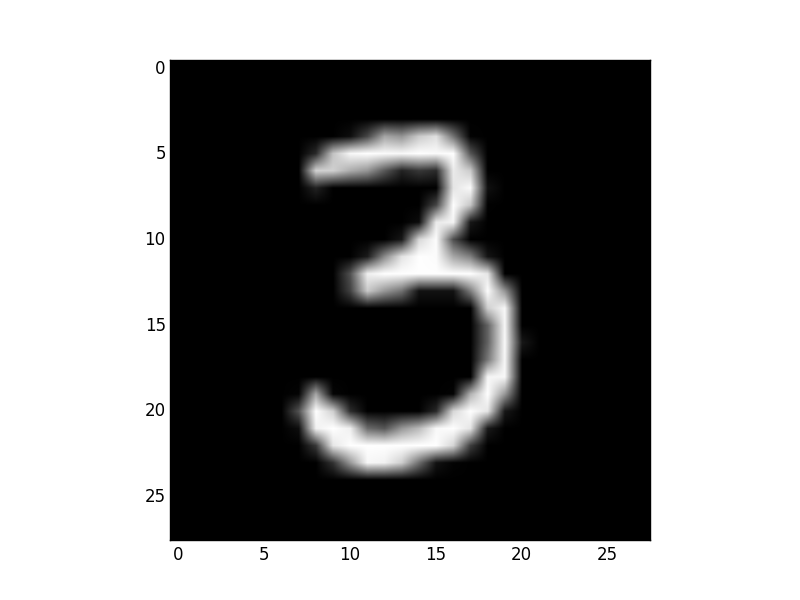
\includegraphics[scale=0.20]{representative-9-2}
    \caption{Class 10 for $K=10$}
\end{figure}

\subsubsection*{Representative images selection}

The way I selected representative images has three steps, with the purposes of fast performance and representatives -

\begin{enumerate}
    \item Filter all images ($X$ values) that clustered to this class, calculate the mean and variance of all these images
    \item Loop through filtered images from beginning, if the distance of this image to mean image is smaller than variance, then select it
    \item once selected images reach $D$ (parameters), break the loop
\end{enumerate}

Reasoning: 
\begin{enumerate}
    \item The optimized method is to filter out all images, calculate all their differences, sort them and select those with minimum values. But this cost a lot of time on sorting and calculating differences while useless if $D$ is small, so I only loop from beginning and break the loop if $D$ is reached
    \item Also this way can help derive some mistaken plot, which would be helpful to research what kind of patterns making the class clustering not well, e.g. $9$ and $4$ are easy mixed, $8$ and $3$ are easy mixed, if selecting the best representatives, we can't find this.
\end{enumerate}

\subsubsection*{Different $K$'s}

Let's try some small $K$'s, Figure 13 - 14 are the results for $K=2$,

\begin{figure}[ht]
    \centering
    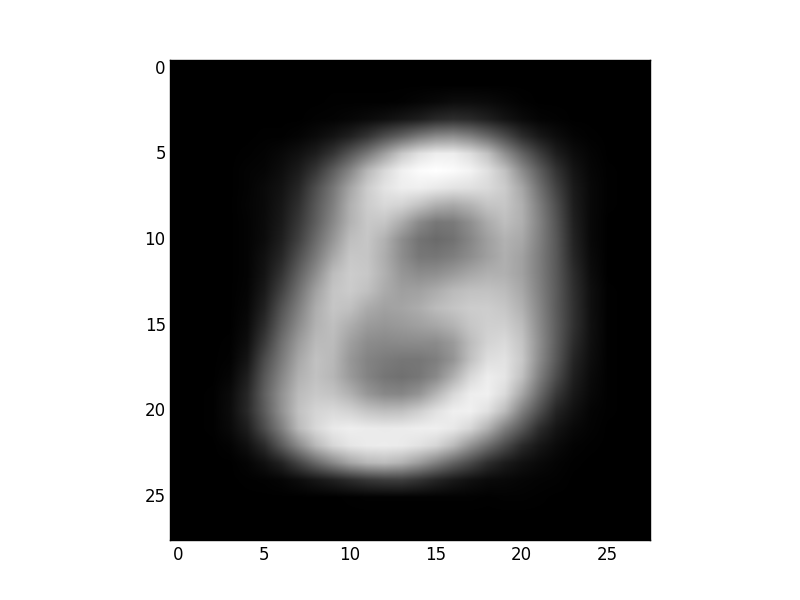
\includegraphics[scale=0.15]{K2-mean-0}
    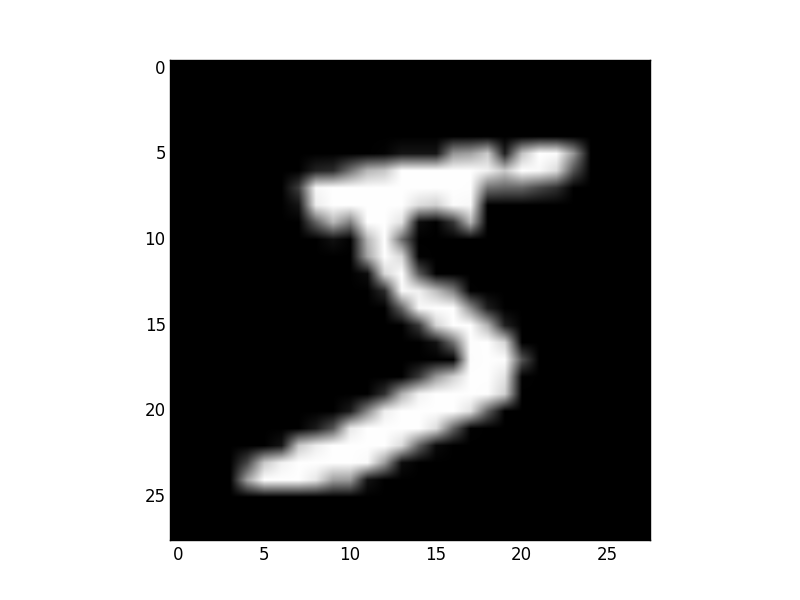
\includegraphics[scale=0.15]{K2-representative-0-0}
    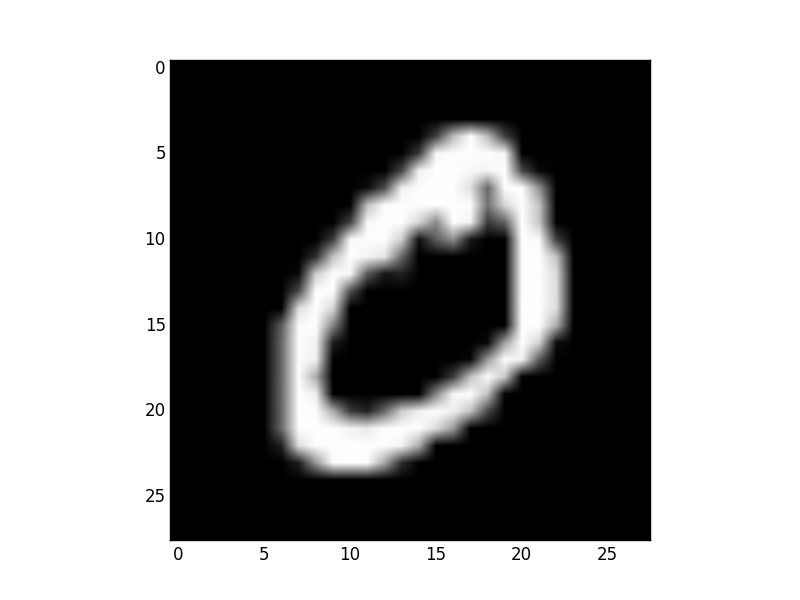
\includegraphics[scale=0.15]{K2-representative-0-1}
    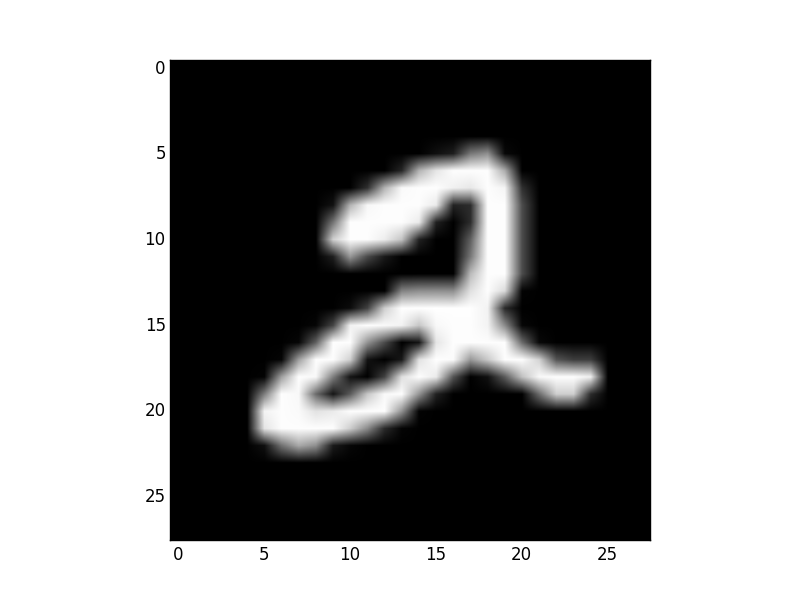
\includegraphics[scale=0.15]{K2-representative-0-2}
    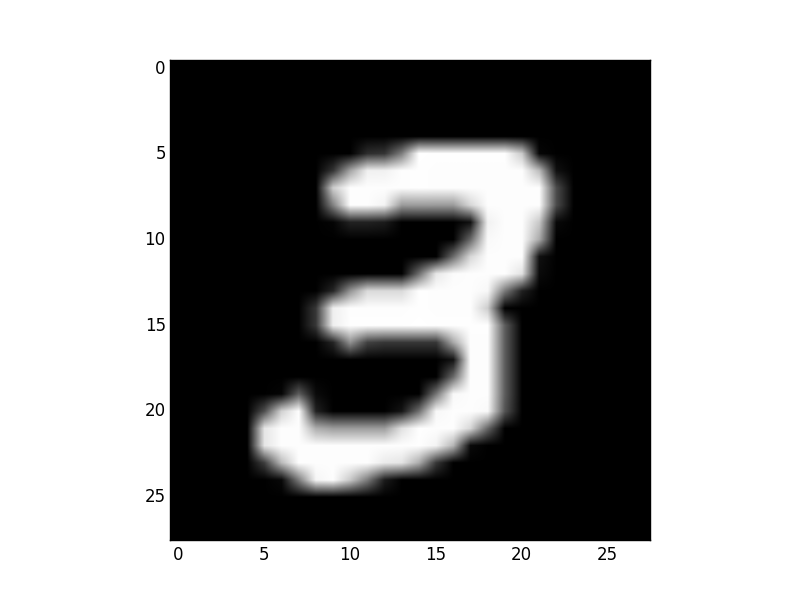
\includegraphics[scale=0.15]{K2-representative-0-3}
    \caption{Class 1 for $K=2$}
\end{figure}

\begin{figure}[ht]
    \centering
    \includegraphics[scale=0.15]{K2-mean-1}
    \includegraphics[scale=0.15]{K2-representative-1-0}
    \includegraphics[scale=0.15]{K2-representative-1-1}
    \includegraphics[scale=0.15]{K2-representative-1-2}
    \includegraphics[scale=0.15]{K2-representative-1-3}
    \caption{Class 2 for $K=2$}
\end{figure}

Figure 15 - 17 are the results for $K=3$,

\begin{figure}[ht]
    \centering
    \includegraphics[scale=0.15]{K3-mean-0}
    \includegraphics[scale=0.15]{K3-representative-0-0}
    \includegraphics[scale=0.15]{K3-representative-0-1}
    \includegraphics[scale=0.15]{K3-representative-0-2}
    \includegraphics[scale=0.15]{K3-representative-0-3}
    \caption{Class 1 for $K=3$}
\end{figure}

\begin{figure}[ht]
    \centering
    \includegraphics[scale=0.15]{K3-mean-1}
    \includegraphics[scale=0.15]{K3-representative-1-0}
    \includegraphics[scale=0.15]{K3-representative-1-1}
    \includegraphics[scale=0.15]{K3-representative-1-2}
    \includegraphics[scale=0.15]{K3-representative-1-3}
    \caption{Class 2 for $K=3$}
\end{figure}

\begin{figure}[ht]
    \centering
    \includegraphics[scale=0.15]{K3-mean-2}
    \includegraphics[scale=0.15]{K3-representative-2-0}
    \includegraphics[scale=0.15]{K3-representative-2-1}
    \includegraphics[scale=0.15]{K3-representative-2-2}
    \includegraphics[scale=0.15]{K3-representative-2-3}
    \caption{Class 3 for $K=3$}
\end{figure}

\subsubsection*{Difference for different restarts and / or different $K$}
Different restarts will generate results differently but will not be wildly different, because it chooses $k$ observations (rows) at random from data for the initial centroids, however the final results should be similar.

For different $K$, as shown above as a comparisons between $K=10,2,3$, the results are wildly different obviously, especially when the difference of $K$ is large.

\subsubsection*{Plot K-means objective function vs. iteration}

Figure 18 is the plot of K-means object function vs. iteration (one example of $K=3$). Obviously it never increases, verified.

\begin{figure}[ht]
    \centering
    \includegraphics[scale=0.5]{prob3}
    \caption{K-means objective function vs. iteration}
\end{figure}

\subsubsection*{K-means++}

Figure 19 - 28 are the results of K-means++ for $K=10$, obviously the result is similar (a little bit better) to K-means. Though it does not give me more obvious satisfying initializations, K-means++ selects initial cluster centers for k-mean clustering in a smart way, which speeds up the convergence a lot, with a half of the running time (22.5s) compared to originals (52.3s).

\begin{figure}[ht]
    \centering
    \includegraphics[scale=0.20]{K10-mean-0}
    \includegraphics[scale=0.20]{K10-representative-0-0}
    \includegraphics[scale=0.20]{K10-representative-0-1}
    \includegraphics[scale=0.20]{K10-representative-0-2}
    \caption{Class 1 for K-means++ $K=10$}
\end{figure}

\begin{figure}[ht]
    \centering
    \includegraphics[scale=0.20]{K10-mean-1}
    \includegraphics[scale=0.20]{K10-representative-1-0}
    \includegraphics[scale=0.20]{K10-representative-1-1}
    \includegraphics[scale=0.20]{K10-representative-1-2}
    \caption{Class 2 for K-means++ $K=10$}
\end{figure}

\begin{figure}[ht]
    \centering
    \includegraphics[scale=0.20]{K10-mean-2}
    \includegraphics[scale=0.20]{K10-representative-2-0}
    \includegraphics[scale=0.20]{K10-representative-2-1}
    \includegraphics[scale=0.20]{K10-representative-2-2}
    \caption{Class 3 for K-means++ $K=10$}
\end{figure}

\begin{figure}[ht]
    \centering
    \includegraphics[scale=0.20]{K10-mean-3}
    \includegraphics[scale=0.20]{K10-representative-3-0}
    \includegraphics[scale=0.20]{K10-representative-3-1}
    \includegraphics[scale=0.20]{K10-representative-3-2}
    \caption{Class 4 for K-means++ $K=10$}
\end{figure}

\begin{figure}[ht]
    \centering
    \includegraphics[scale=0.20]{K10-mean-4}
    \includegraphics[scale=0.20]{K10-representative-4-0}
    \includegraphics[scale=0.20]{K10-representative-4-1}
    \includegraphics[scale=0.20]{K10-representative-4-2}
    \caption{Class 5 for K-means++ $K=10$}
\end{figure}

\begin{figure}[ht]
    \centering
    \includegraphics[scale=0.20]{K10-mean-5}
    \includegraphics[scale=0.20]{K10-representative-5-0}
    \includegraphics[scale=0.20]{K10-representative-5-1}
    \includegraphics[scale=0.20]{K10-representative-5-2}
    \caption{Class 6 for K-means++ $K=10$}
\end{figure}

\begin{figure}[ht]
    \centering
    \includegraphics[scale=0.20]{K10-mean-6}
    \includegraphics[scale=0.20]{K10-representative-6-0}
    \includegraphics[scale=0.20]{K10-representative-6-1}
    \includegraphics[scale=0.20]{K10-representative-6-2}
    \caption{Class 7 for K-means++ $K=10$}
\end{figure}

\begin{figure}[ht]
    \centering
    \includegraphics[scale=0.20]{K10-mean-7}
    \includegraphics[scale=0.20]{K10-representative-7-0}
    \includegraphics[scale=0.20]{K10-representative-7-1}
    \includegraphics[scale=0.20]{K10-representative-7-2}
    \caption{Class 8 for K-means++ $K=10$}
\end{figure}

\begin{figure}[ht]
    \centering
    \includegraphics[scale=0.20]{K10-mean-8}
    \includegraphics[scale=0.20]{K10-representative-8-0}
    \includegraphics[scale=0.20]{K10-representative-8-1}
    \includegraphics[scale=0.20]{K10-representative-8-2}
    \caption{Class 9 for K-means++ $K=10$}
\end{figure}

\begin{figure}[ht]
    \centering
    \includegraphics[scale=0.20]{K10-mean-9}
    \includegraphics[scale=0.20]{K10-representative-9-0}
    \includegraphics[scale=0.20]{K10-representative-9-1}
    \includegraphics[scale=0.20]{K10-representative-9-2}
    \caption{Class 10 for K-means++ $K=10$}
\end{figure}

\newpage
\begin{problem}[Calibration, 1pt]
Approximately how long did this homework take you to complete?
\end{problem}
\subsection*{Solution}
6 hours.

\end{document}
